% !TEX program = tectonic
% Deck AUTONOME « La donnée de la Chambre, de bout en bout » (House 2013-2026).
% Format repris de SLIDES_DONNEES_S1S2_V2.tex : thème Madrid, mécanisme \pipefig (carte
% unique du trajet, une seule étape allumée), \choixbox, \repband, \partdivider.
%
% BUT (demande d'Alice, 2026-07-21) : qu'après lecture on ait VRAIMENT compris la donnée.
% Quatre exigences, qui commandent le plan :
%   (1) chaque chiffre est DÉCOMPOSABLE — aucun total sans ses parties, et la somme boucle ;
%   (2) tous les CHOIX de traitement sont énoncés, chiffrés, avec l'autre option quand elle est mesurée ;
%   (3) ce qui reste INEXPLOITÉ est dit, en lignes / dollars / membres ;
%   (4) ce que la donnée PERMET et NE PERMET PAS pour une stratégie.
%
% SOURCE UNIQUE DES CHIFFRES : 01_autres_filing_types/Portefeuilles_House_Complet.ipynb (158 cellules,
% toutes exécutées). Aucun chiffre de ce deck n'est écrit à la main : chacun sort d'une cellule.
% La fiche FICHE_DONNEES_HOUSE.pdf est le résumé 4 pages du même contenu — mêmes chiffres.
% Figures : ../figures/fig_10_*.png, produites par ce même notebook.
%
% Additif : ne modifie ni le notebook, ni la fiche, ni les autres decks.
\documentclass[11pt,aspectratio=169]{beamer}
\definecolor{helec}{HTML}{3B6EA5}   % couleur maîtresse
\usetheme{Madrid}
\usecolortheme[named=helec]{structure}
\setbeamertemplate{navigation symbols}{}
\setbeamertemplate{blocks}[rounded][shadow=false]
\setbeamerfont{frametitle}{series=\bfseries}
\usepackage[T1]{fontenc}
\usepackage{lmodern}
\usepackage[utf8]{inputenc}
\usepackage[french]{babel}
\usepackage{booktabs}
\usepackage{xcolor}
\usepackage{graphicx}
\usepackage{amssymb}
\usepackage{amsmath}
\usepackage{array}
\usepackage{newunicodechar}
\usepackage{tikz}
\usetikzlibrary{arrows.meta,positioning,calc}
\hypersetup{colorlinks=true, urlcolor=helec, linkcolor=white}
\graphicspath{{../figures/}{figs/}}

% Caractères Unicode → commandes (fontes T1)
\newunicodechar{→}{\ensuremath{\rightarrow}}
\newunicodechar{—}{\textemdash}
\newunicodechar{–}{\textendash}
\newunicodechar{…}{\ldots}
\newunicodechar{·}{\textperiodcentered}
\newunicodechar{≈}{\ensuremath{\approx}}
\newunicodechar{×}{\ensuremath{\times}}
\newunicodechar{≤}{\ensuremath{\leq}}
\newunicodechar{≥}{\ensuremath{\geq}}
\newunicodechar{−}{\ensuremath{-}}
\newunicodechar{±}{\ensuremath{\pm}}
\newunicodechar{✓}{\checkmark}
\newunicodechar{↔}{\ensuremath{\leftrightarrow}}
\newunicodechar{≠}{\ensuremath{\neq}}
\newunicodechar{⊇}{\ensuremath{\supseteq}}
\newunicodechar{⊂}{\ensuremath{\subset}}
\newunicodechar{∑}{\ensuremath{\textstyle\sum}}
\newunicodechar{∧}{\ensuremath{\wedge}}
\newunicodechar{⇒}{\ensuremath{\Rightarrow}}
\newunicodechar{œ}{\oe}
\newunicodechar{Œ}{\OE}
\newunicodechar{°}{\textdegree}
\newunicodechar{§}{\S}
\newunicodechar{«}{\og}
\newunicodechar{»}{\fg{}}

% ── Code couleur ──
% Le deck n'a que deux familles : ce que le MEMBRE dépose (bleu), ce que NOUS en faisons (vert).
% L'ocre marque la donnée intermédiaire, le rouge un choix ou une alerte.
\definecolor{helec}{HTML}{3B6EA5}     % bleu — l'acte I : le membre dépose
\definecolor{hocr}{HTML}{A9C5E2}      % bleu clair — la voie scannée (OCR)
\definecolor{okgreen}{HTML}{2E8B57}   % vert — l'acte II : ce qu'on en fait
\definecolor{alertred}{HTML}{C0392B}
\definecolor{warnorange}{HTML}{E67E22}
\definecolor{dataC}{RGB}{176,110,14}  % ocre — la donnée en transit
\definecolor{grisC}{RGB}{90,90,90}

\newcommand{\co}[1]{\texttt{#1}}
\tikzset{
  step/.style={rectangle, rounded corners=2pt, draw=#1, line width=0.8pt, fill=#1!8,
               align=center, font=\scriptsize, minimum height=0.72cm},
  bande/.style={rectangle, rounded corners=2pt, draw=#1, line width=0.8pt, fill=#1!8,
                align=center, font=\scriptsize, minimum height=0.62cm},
  arr/.style={-{Latex[length=2mm]}, line width=0.8pt, draw=gray!65},
}

\newcommand{\badge}[2]{\colorbox{#1}{\textcolor{white}{\footnotesize\textbf{#2}}}}
\newcommand{\badgel}[2]{\colorbox{#1}{\textcolor{black!80}{\footnotesize\textbf{#2}}}}
\newcommand{\kpi}[3]{{\large\textbf{\textcolor{#1}{#2}}}~{\footnotesize #3}}
\newcommand{\defl}[1]{{\scriptsize\color{black!55}#1}}

% Carreau chiffre-clé : \tuile{couleur}{gros chiffre}{légende}
\newcommand{\tuile}[3]{%
  \begin{minipage}[t]{0.23\textwidth}\centering
    \colorbox{#1}{\parbox[c][20mm][c]{\dimexpr\linewidth-8pt}{\centering
      {\color{white}\Large\textbf{#2}}\\[0.5mm]{\color{white}\footnotesize #3}}}
  \end{minipage}}

% Encadré CHOIX : une décision de traitement, ce qu'elle déplace, ce que l'autre option donnerait.
\newcommand{\choixbox}[1]{%
  \colorbox{alertred!8}{\parbox{\dimexpr\linewidth-8pt}{\scriptsize
    \textbf{\textcolor{alertred}{CHOIX}}\; --- #1}}}
% Bandeau RÉPONSE : la conclusion d'une partie, en une phrase.
\newcommand{\repband}[1]{%
  \colorbox{okgreen!12}{\parbox{\dimexpr\textwidth-10pt}{\scriptsize
    \textbf{\textcolor{okgreen}{Réponse}}\; --- #1}}}
% Bandeau PIÈGE : une confusion à ne pas faire (deux chiffres qui se ressemblent, un mot polysémique).
\newcommand{\piege}[1]{%
  \colorbox{warnorange!12}{\parbox{\dimexpr\linewidth-8pt}{\scriptsize
    \textbf{\textcolor{warnorange}{PIÈGE}}\; --- #1}}}

% Bande maths : \bmaths{noms des termes}{formule sur une ligne}
\newcommand{\bmaths}[2]{%
  {\scriptsize\color{black!55}#1}\\[0.2mm]
  {\small$\displaystyle #2$}\\[2mm]}

% Séparateur de partie plein cadre : \partdivider{couleur}{PARTIE X}{Grand titre}{sous-titre}
\newcommand{\partdivider}[4]{%
  {\setbeamercolor{background canvas}{bg=#1}
  \begin{frame}[plain]
    \centering\vfill
    {\color{white}\Large\textbf{#2}}\\[3.5mm]
    {\color{white!75}\rule{0.40\textwidth}{1pt}}\\[4.5mm]
    {\color{white}\fontsize{32}{36}\selectfont\textbf{#3}}\\[5.5mm]
    {\color{white!88}\large #4}
    \vfill
  \end{frame}}}
% Intercalaire de chapitre : \chapdivider{label}{Grand titre}{sous-titre}
\newcommand{\chapdivider}[3]{%
  \begin{frame}[plain]
    \centering\vfill
    {\color{helec!85}\large\textbf{#1}}\\[3.5mm]
    {\color{black!88}\fontsize{29}{33}\selectfont\textbf{#2}}\\[4mm]
    {\color{helec!45}\rule{0.30\textwidth}{1.2pt}}\\[4mm]
    {\color{black!55}\large #3}
    \vfill
  \end{frame}}

% Ligne d'étape dans un sommaire : \etape{n}{titre}{glose}
\newcommand{\etape}[3]{%
  {\color{helec}\bfseries #1}\; & \textbf{#2} & {\scriptsize\color{black!60} #3}\\[0.6mm]}

% ════════════════════════════════════════════════════════════════════════════════
%  LA CARTE — dessin unique du trajet, réutilisé à chaque étape
% ════════════════════════════════════════════════════════════════════════════════
% \pipefig{k} : k = 0 → tout allumé (vue d'ensemble) ; k = 1..9 → seule l'étape k est allumée,
% le reste est estompé à 16 %. Même dessin à chaque fois, seul le curseur bouge.
%
% Le trajet a deux moitiés, et la carte le montre :
%   ACTE I (bleu, étapes 1-4) — ce que le MEMBRE dépose, dans l'ordre de son mandat :
%       1 il arrive · 2 il trade · 3 il déclare · 4 il part
%   la CHARNIÈRE — les dépôts ne portent pas une matière mais DEUX : des positions
%       (Schedule A : ce qu'il possède) et des transactions (Schedule B : ce qu'il a échangé).
%       Cette séparation commande tout l'aval : les positions donnent le point de départ et
%       servent de juge, les transactions font bouger le portefeuille.
%   ACTE II (vert, étapes 5-9) — ce que NOUS en faisons :
%       5 rassembler · 6 trier · 7 valoriser · 8 reconstruire · 9 vérifier
%
% Correspondance étape → bandes du dessin (les lettres nomment les BANDES, pas les étapes) :
%   1 = \opA (arrivée)      4 = \opD (sortie)        7 = \opG (valoriser)
%   2 = \opB (fil de l'eau) 5 = \opE (rassembler)    8 = \opH (reconstruire)
%   3 = \opC (annuel)       6 = \opF (trier)         9 = \opI (vérifier)
%   \opS = la charnière A/B — allumée en 1, 2, 3, 4 (elle explique ce que chaque dépôt porte)
%          et en vue d'ensemble.
\newcommand{\pipefig}[1]{%
  \def\opA{0.16}\def\opB{0.16}\def\opC{0.16}\def\opD{0.16}\def\opS{0.16}%
  \def\opE{0.16}\def\opF{0.16}\def\opG{0.16}\def\opH{0.16}\def\opI{0.16}%
  \ifnum#1=0 \def\opA{1}\def\opB{1}\def\opC{1}\def\opD{1}\def\opS{1}%
             \def\opE{1}\def\opF{1}\def\opG{1}\def\opH{1}\def\opI{1}\fi
  \ifnum#1=1 \def\opA{1}\def\opS{1}\fi
  \ifnum#1=2 \def\opB{1}\def\opS{1}\fi
  \ifnum#1=3 \def\opC{1}\def\opS{1}\fi
  \ifnum#1=4 \def\opD{1}\def\opS{1}\fi
  \ifnum#1=5 \def\opE{1}\fi  \ifnum#1=6 \def\opF{1}\fi  \ifnum#1=7 \def\opG{1}\fi
  \ifnum#1=8 \def\opH{1}\fi  \ifnum#1=9 \def\opI{1}\fi
  \begin{tikzpicture}[node distance=3mm, every node/.style={transform shape}]
    % ═══ ACTE I — les quatre moments du mandat ═══
    \node[font=\tiny\bfseries, text=helec!80, align=left] at (-8.2,0.75)
      {ACTE I\\le membre\\dépose};
    \begin{scope}[opacity=\opA, text opacity=\opA]
      \node[step=helec, text width=2.9cm] (arr) at (-4.9,0.75)
        {\textbf{1 · IL ARRIVE}\\{\tiny entrée \emph{H} · candidature \emph{C}}};
    \end{scope}
    \begin{scope}[opacity=\opB, text opacity=\opB]
      \node[step=helec, text width=2.9cm] (fil) at (-1.6,0.75)
        {\textbf{2 · IL TRADE}\\{\tiny déclaration rapide \emph{P}}};
    \end{scope}
    \begin{scope}[opacity=\opC, text opacity=\opC]
      \node[step=helec, text width=2.9cm] (ann) at (1.7,0.75)
        {\textbf{3 · IL DÉCLARE}\\{\tiny rapport annuel \emph{O} · \emph{A}}};
    \end{scope}
    \begin{scope}[opacity=\opD, text opacity=\opD]
      \node[step=helec, text width=2.9cm] (sor) at (5.0,0.75)
        {\textbf{4 · IL PART}\\{\tiny sortie \emph{T}}};
    \end{scope}
    % ═══ LA CHARNIÈRE — un dépôt porte deux matières ═══
    % Les pastilles disent quel moment alimente quelle matière : cinq flèches croisées
    % seraient illisibles sur une carte relue dix fois. Les moments 3 et 4 figurent des DEUX
    % côtés — le rapport annuel, l'amendement et la sortie portent les deux sections, alors
    % que l'arrivée (1) ne porte que des positions et la déclaration rapide (2) que des
    % transactions. C'est le point à retenir de la charnière.
    \begin{scope}[opacity=\opS, text opacity=\opS]
      \node[step=dataC, text width=5.9cm] (schA) at (-3.2,-1.15)
        {\textbf{POSITIONS} --- \emph{Schedule A} \;\colorbox{helec!22}{\tiny\textbf{1·3·4}}\\
         {\tiny ce qu'il possède, à une date}};
      \node[step=dataC, text width=5.9cm] (schB) at (3.3,-1.15)
        {\textbf{TRANSACTIONS} --- \emph{Sch. B} \;\colorbox{helec!22}{\tiny\textbf{2·3·4}}\\
         {\tiny ce qu'il a acheté ou vendu}};
      \node[font=\scriptsize, text=black!60, align=center, text width=13.4cm] at (0,-2.15)
        {les positions donnent le \textbf{point de départ} et servent de \textbf{juge}\\
         les transactions \textbf{font bouger} le portefeuille};
    \end{scope}
    % ═══ ACTE II — ce que nous en faisons ═══
    \node[font=\tiny\bfseries, text=okgreen!80, align=left] at (-8.2,-3.9)
      {ACTE II\\ce qu'on\\en fait};
    \begin{scope}[opacity=\opE, text opacity=\opE]
      \node[bande=okgreen, text width=12.2cm] (ras) at (0,-3.05)
        {\textbf{5 · RASSEMBLER} --- réunir tous les dépôts, compter ce qu'ils contiennent};
    \end{scope}
    \begin{scope}[opacity=\opF, text opacity=\opF]
      \node[bande=okgreen, text width=12.2cm] (tri) at (0,-3.85)
        {\textbf{6 · TRIER} --- chaque ligne reçoit sa classe \emph{avant} tout prix :
         action, fonds, monétaire, code de formulaire};
    \end{scope}
    \begin{scope}[opacity=\opG, text opacity=\opG]
      \node[bande=okgreen, text width=12.2cm] (val) at (0,-4.65)
        {\textbf{7 · VALORISER} --- ne garder que les transactions dont on connaît
         le \textbf{prix du jour}};
    \end{scope}
    \begin{scope}[opacity=\opH, text opacity=\opH]
      \node[bande=okgreen, fill=okgreen!16, text width=12.2cm] (rec) at (0,-5.45)
        {\textbf{8 · RECONSTRUIRE} --- la photo devient un portefeuille en \textbf{parts},
         les transactions le font vivre};
    \end{scope}
    \begin{scope}[opacity=\opI, text opacity=\opI]
      \node[bande=helec, fill=helec!16, text width=12.2cm] (ver) at (0,-6.35)
        {\textbf{9 · VÉRIFIER} --- les \textbf{positions} des rapports annuels, qui n'ont
         jamais servi à construire, jugent le portefeuille};
    \end{scope}
    % ═══ les flèches ═══
    % De la rangée des moments vers la charnière : une flèche par moment, verticale et courte.
    % La répartition A / B est portée par les pastilles, pas par des traits croisés.
    \begin{scope}[opacity=0.30]
      \draw[arr] (arr.south) -- ++(0,-0.30);
      \draw[arr] (fil.south) -- ++(0,-0.30);
      \draw[arr] (ann.south) -- ++(0,-0.30);
      \draw[arr] (sor.south) -- ++(0,-0.30);
      \draw[arr] (schA.south) -- (ras.north -| schA.south);
      \draw[arr] (schB.south) -- (ras.north -| schB.south);
      \draw[arr] (ras) -- (tri); \draw[arr] (tri) -- (val);
      \draw[arr] (val) -- (rec); \draw[arr] (rec) -- (ver);
    \end{scope}
  \end{tikzpicture}}

% Slide-repère « vous êtes ici » : \pipeslide{k}{titre}{la question}{ce qu'on en sort}
\newcommand{\pipeslide}[4]{%
  \begin{frame}{#2}
    \centering
    \resizebox{!}{0.63\textheight}{\pipefig{#1}}\\[2mm]
    \colorbox{helec!10}{\parbox{0.94\textwidth}{\centering\footnotesize\vspace{0.5mm}
      \emph{#3}\\[0.8mm]{\scriptsize\color{black!65} ce qu'on en sort : #4}\vspace{0.5mm}}}
  \end{frame}}
% Bandeau réduit : la carte en tête d'une frame de contenu, pour ne jamais perdre le fil.
\newcommand{\pipestrip}[1]{\resizebox{0.86\textwidth}{!}{\pipefig{#1}}}

\title[La donnée de la Chambre]{\textbf{La donnée de la Chambre, de bout en bout}}
\subtitle{Ce qu'ils déposent, ce qu'on en fait, ce qu'on peut en tirer}
\author{}
\date{}

\begin{document}

% ═══════════ part0 ═══════════
% ════════════════════════════════════════════════════════════════════════════════
%  PART 0 — OUVERTURE
%  Titre · la question · la carte · le sommaire · le mode d'emploi des chiffres ·
%  les quatre exigences.
%  Tous les chiffres viennent du notebook Portefeuilles_House_Complet (cellules citées).
% ════════════════════════════════════════════════════════════════════════════════

% ── 1 · Page de titre ───────────────────────────────────────────────────────────
\begin{frame}[plain]
  \centering\vfill
  {\color{helec}\fontsize{30}{34}\selectfont\textbf{La donnée de la Chambre,}}\\[1.5mm]
  {\color{helec}\fontsize{30}{34}\selectfont\textbf{de bout en bout}}\\[5mm]
  {\color{helec!45}\rule{0.42\textwidth}{1.2pt}}\\[5mm]
  {\color{black!70}\large Ce qu'ils déposent, ce qu'on en fait, ce qu'on peut en tirer}\\[3mm]
  {\color{black!45}\footnotesize Chambre des représentants · transactions 2013--2026}\\[8mm]
  \colorbox{helec!8}{\parbox{0.84\textwidth}{\centering\footnotesize\vspace{1mm}
    À la fin de ce document, vous saurez d'où vient chacune des \textbf{129\,538} transactions
    reconstituées, ce qui manque à celles qu'on ne reconstruit pas,
    et ce que cette donnée autorise --- ou interdit --- à une stratégie.\vspace{1mm}}}
  \vfill
\end{frame}

% ── 2 · La question ─────────────────────────────────────────────────────────────
\begin{frame}{De quoi dispose-t-on exactement, et que peut-on en faire ?}
  \begin{columns}[T]
    \begin{column}{0.50\textwidth}
      \footnotesize
      Deux questions, dans cet ordre, et jamais mélangées :
      \begin{itemize}\itemsep2.5pt
        \item \textbf{de quoi dispose-t-on ?} --- quels documents un membre dépose,
              ce qu'ils contiennent, ce qu'on arrive à en lire ;
        \item \textbf{que peut-on en faire ?} --- ce qu'on reconstruit avec,
              ce que la reconstruction rate, et ce qui reste hors d'atteinte.
      \end{itemize}
      \vspace{2mm}
      \defl{Ce document décrit la donnée. Il ne juge aucune performance.}
    \end{column}
    \begin{column}{0.46\textwidth}
      \footnotesize\raggedright
      \kpi{helec}{900}{membres au registre}\\
      \defl{toute personne ayant siégé à la Chambre entre 2013 et 2026,
        d'après le référentiel officiel des mandats (couverture 900/900)}\\[2.5mm]
      \kpi{dataC}{609\,886}{lignes de patrimoine déposées}\\
      \defl{dépôts 2014--2026, empilés : le même actif revient à chaque
        déclaration --- ce n'est pas un patrimoine, on le décompose plus loin}\\[2.5mm]
      \kpi{okgreen}{129\,538}{transactions retenues}\\
      \defl{2013--2026 : ce qu'on arrive à rejouer, chez 408 membres}
    \end{column}
  \end{columns}
  \vspace{2.5mm}
  \colorbox{black!5}{\parbox{\dimexpr\textwidth-8pt}{\scriptsize\vspace{0.5mm}
    \textbf{D'où vient tout ce qui suit.} Un seul notebook, toutes cellules exécutées, une seule
    exécution : \co{Portefeuilles\_House\_Complet}. Chaque chiffre de ce deck est recopié d'une
    sortie de cellule identifiée, et chaque figure est produite par le même notebook ; aucun n'est
    estimé, arrondi à la volée, ni recopié d'un document antérieur. Les seules données héritées
    sont \textbf{quatre tables v1 gelées} --- registre des membres 900 $\times$ 10, positions
    420\,916 $\times$ 12, flux des rapports 26\,115 $\times$ 28, photos d'entrée 284 $\times$ 7 ---
    rechargées et recomptées ici.\vspace{0.5mm}}}
\end{frame}

% ── 3 · La carte d'ensemble ─────────────────────────────────────────────────────
\begin{frame}{Quatre moments de dépôt, deux matières, cinq traitements}
  \centering
  \resizebox{0.80\textwidth}{!}{\pipefig{0}}\\[1mm]
  {\scriptsize\color{black!55} \emph{A} = amendement, la version corrigée d'un dépôt déjà remis
  --- cette même carte revient à chaque étape, avec une seule case allumée}
\end{frame}

% ── 4 · Le sommaire ─────────────────────────────────────────────────────────────
\begin{frame}{Deux actes, neuf étapes}
  \centering\small
  \begin{tabular}{@{}c@{\hspace{2.5mm}}l@{\hspace{3mm}}l@{}}
    \multicolumn{3}{@{}l}{\textcolor{helec}{\footnotesize\textbf{ACTE I — le membre dépose}}}\\[0.6mm]
    \etape{1}{Il arrive}{sa photo d'entrée \emph{H}, ou sa candidature \emph{C} : ce qu'il possède au départ}
    \etape{2}{Il trade}{la déclaration rapide \emph{P}, une transaction à la fois}
    \etape{3}{Il déclare}{le rapport annuel \emph{O}, ou son amendement \emph{A} :
      ses positions \emph{et} ses transactions de l'année}
    \etape{4}{Il part}{sa photo de sortie \emph{T} : le dernier état connu}
    \multicolumn{3}{@{}l}{\parbox{0.95\textwidth}{\raggedright
      \hspace{1mm}\textcolor{dataC}{\scriptsize\textbf{la charnière}} \;
      {\scriptsize\color{black!60} un formulaire de patrimoine a deux sections : des
      \emph{positions} (Schedule A) et des \emph{transactions} (Schedule B). La déclaration
      rapide \emph{P} ne porte que des transactions ; \emph{H} et \emph{C} que des positions ;
      \emph{O}, \emph{A} et \emph{T} portent les deux.}}}\\[0.4mm]
    \multicolumn{3}{@{}l}{\textcolor{okgreen}{\footnotesize\textbf{ACTE II — ce qu'on en fait}}}\\[0.6mm]
    \etape{5}{On rassemble}{réunir le flux électronique et les documents scannés, et compter}
    \etape{6}{On trie}{chaque ligne reçoit sa classe --- action, fonds, monétaire, code de
      formulaire --- \emph{avant} tout prix}
    \etape{7}{On valorise}{ne garder que ce dont on connaît le prix du jour}
    \etape{8}{On reconstruit}{\parbox[t]{0.72\textwidth}{\raggedright la photo devient un
      portefeuille en \emph{parts} --- une valeur de part qui démarre à 1, comme un fonds ---
      et les transactions le font vivre}}
    \etape{9}{On vérifie}{\parbox[t]{0.72\textwidth}{\raggedright les \emph{positions} des rapports
      annuels (Schedule A), jamais utilisées pour construire, jugent le portefeuille reconstruit ;
      leurs \emph{transactions} (Schedule B), elles, ont servi à le construire}}
  \end{tabular}\\[0.2mm]
  {\scriptsize\color{black!60} Puis trois parties : \textbf{les choix qu'on a faits} (chaque
  décision, son volume, l'autre option), \textbf{ce qui reste} (l'inexploité, le fragile,
  l'inexistant), \textbf{ce qu'on peut en faire}.}
\end{frame}

% ── 5 · Le mode d'emploi des chiffres ───────────────────────────────────────────
\begin{frame}{Quatre niveaux de comptage, à ne jamais confondre}
  \centering\scriptsize
  \begin{tabular}{@{}l l r >{\raggedright\arraybackslash}p{6.8cm}@{}}
    \toprule
    \textbf{niveau} & \textbf{ce que c'est} & \textbf{ici} & \textbf{et de quoi c'est fait}\\
    \midrule
    \textcolor{helec}{\textbf{un DÉPÔT-PHOTO}} & un document de patrimoine & 6\,135 &
      chez 887 déposants (875 membres du registre + 12 candidats jamais élus) :\newline
      4\,447 annuels \emph{O} + 934 candidatures \emph{C}
      + 378 sorties \emph{T} + 376 entrées \emph{H}\\[1.1mm]
    \textcolor{dataC}{\textbf{une LIGNE}} & une ligne \emph{dans} un document & 609\,886 &
      lignes de positions, issues de 14\,887 documents :\newline
      420\,916 (électronique) + 188\,970 (scanné, océrisé)\\[1.1mm]
    \textcolor{okgreen}{\textbf{une TRANSACTION}} & un achat ou une vente & 129\,538 &
      transactions retenues :\newline 107\,976 (déclarations rapides)
      + 14\,084 (rapports, amendements et sorties, flux électronique)
      + 7\,478 (les mêmes, en papier océrisé)\\[1.1mm]
    \textcolor{alertred}{\textbf{un MEMBRE}} & une personne du registre & 900 &
      personnes ayant siégé entre 2013 et 2026 :\newline 305 vus par les déclarations rapides
      + 103 vus seulement par les rapports + 492 sans trade exploitable\\
    \bottomrule
  \end{tabular}\\[1.2mm]
  {\scriptsize\color{black!60} Hors de ces 6\,135 photos : les déclarations rapides \emph{P}
  (5\,571 dépôts, aucune position) et 139 amendements \emph{A} porteurs de transactions inédites.}\\[1.5mm]
  \piege{une ligne n'est pas un avoir. Les 609\,886 lignes empilent le \emph{même} actif re-déclaré
  chaque année : additionnées elles pèsent 104\,130 M\$, quand le dernier document de chaque membre
  ne vaut que 8\,887 M\$ --- \textbf{12 fois moins}. Le premier total ne nomme rien de réel.}
\end{frame}

% ── 6 · Les quatre exigences ────────────────────────────────────────────────────
\begin{frame}{Ce que ce document s'engage à faire}
  \centering\footnotesize
  \begin{tabular}{@{}l p{8.4cm}@{}}
    \toprule
    \textcolor{helec}{\textbf{1 · DÉCOMPOSER}} &
      aucun total n'est donné sans ses parties, et la somme boucle. On doit toujours pouvoir
      demander : « ce chiffre qui reste, il est fait de quoi ? »\\[1.5mm]
    \textcolor{alertred}{\textbf{2 · CHOISIR À VOIX HAUTE}} &
      chaque décision de traitement est énoncée, avec le volume qu'elle déplace --- et l'autre
      option quand elle a été mesurée. Elles portent toutes l'étiquette rouge
      \textcolor{alertred}{\textbf{CHOIX}}.\\[1.5mm]
    \textcolor{warnorange}{\textbf{3 · DIRE CE QUI RESTE}} &
      ce qui n'est pas exploité est chiffré : en lignes, en dollars, en membres --- y compris
      ce qu'on possède déjà et qu'on n'a pas branché.\\[1.5mm]
    \textcolor{okgreen}{\textbf{4 · DIRE CE QUE ÇA PERMET}} &
      ce que la donnée autorise à une stratégie, et ce qu'elle lui interdit : dates de
      publication, granularité des montants, taille de l'échantillon.\\
    \bottomrule
  \end{tabular}\\[3.5mm]
  \piege{ce deck décrit \emph{la donnée}, pas un résultat. Il ne dit jamais si une stratégie est
  rentable --- c'est l'objet d'un autre document.}
\end{frame}

% ═══════════ part1 ═══════════
% ════════════════════════════════════════════════════════════════════════════════
%  ACTE I — ce que le membre dépose, dans l'ordre de son mandat
% ════════════════════════════════════════════════════════════════════════════════
\partdivider{helec}{ACTE I}{Ce qu'ils déposent}{la vie d'un mandat, dans l'ordre}

% ── LA POPULATION ───────────────────────────────────────────────────────────────
\begin{frame}{Le socle de tout le deck : 900 membres, quatre trajectoires}
  \centering
  \begin{tabular}{@{}r@{\;}cc@{}}
    & {\footnotesize\emph{déjà là en 2014} \; \textbf{439}}
    & {\footnotesize\emph{arrivé après 2014} \; \textbf{461}}\\[1mm]
    {\footnotesize\emph{encore en poste} \; \textbf{437}} &
    \colorbox{helec!16}{\parbox[c][13mm][c]{0.34\textwidth}{\centering
      {\Large\textbf{125}}\\[0.4mm]{\footnotesize déjà-là restés}}} &
    \colorbox{okgreen!16}{\parbox[c][13mm][c]{0.34\textwidth}{\centering
      {\Large\textbf{312}}\\[0.4mm]{\footnotesize arrivés restés}}}\\[1.6mm]
    {\footnotesize\emph{parti avant 2026} \; \textbf{463}} &
    \colorbox{helec!8}{\parbox[c][13mm][c]{0.34\textwidth}{\centering
      {\Large\textbf{314}}\\[0.4mm]{\footnotesize déjà-là partis}}} &
    \colorbox{okgreen!8}{\parbox[c][13mm][c]{0.34\textwidth}{\centering
      {\Large\textbf{149}}\\[0.4mm]{\footnotesize cycle complet}}}\\
  \end{tabular}\\[2mm]
  \defl{chaque membre est dans une case et une seule --- était-il en poste au 1\textsuperscript{er} janvier
  2014, l'est-il encore au 1\textsuperscript{er} janvier 2026 ? \quad 125 + 314 + 312 + 149 = \textbf{900}.
  \; Le registre des membres est cadré 2014-2026 ; les transactions, elles, sont cadrées 2013-2026.}\\[3.5mm]
  \kpi{helec}{900}{membres au registre}\qquad
  \kpi{helec}{98,9 \%}{de concordance avec les mandats officiels}\qquad
  \kpi{alertred}{18}{sans document}\\[2mm]
  \defl{98,9 \% = 890 des 900 membres tombent dans la même case selon nos dépôts et selon le
  référentiel officiel des mandats ; les 10 désaccords sont des cas de frontière, listés nommément
  \quad·\quad les 18 sans document : 10 déjà-là partis, 5 arrivés restés,
  2 déjà-là restés, 1 cycle complet}
\end{frame}

\begin{frame}{Sur 900 membres, 408 ont une transaction qu'on sait rejouer}
  \centering
  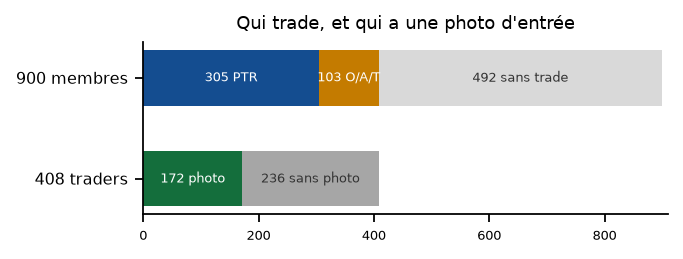
\includegraphics[width=0.58\textwidth]{fig_10_partition.png}\\[0.5mm]
  {\scriptsize\color{black!60} sur la figure : « PTR » = déclaration rapide · « O/A/T » = rapport
  annuel \emph{O} + amendement \emph{A} + sortie \emph{T}.}\\[1.5mm]
  \begin{columns}[t]
    \begin{column}{0.50\textwidth}\footnotesize
      \textbf{Par quel canal on les voit}\\[0.8mm]
      \begin{tabular}{@{}rl@{}}
        \textbf{305} & vus par les déclarations rapides\\
        \textbf{103} & vus seulement par les rapports annuels\\
        \textbf{492} & aucune transaction qu'on sache rejouer\\
        \midrule
        \textbf{900} & membres du registre\\
      \end{tabular}
    \end{column}
    \begin{column}{0.46\textwidth}\footnotesize
      \textbf{Les 408 qui tradent, au départ}\\[0.8mm]
      \begin{tabular}{@{}rl@{}}
        \textbf{172} & ont une photo d'entrée exploitable\\
        \textbf{236} & n'en ont pas : patrimoine nul au départ\\
        \midrule
        \textbf{408} & membres qui tradent\\
      \end{tabular}
    \end{column}
  \end{columns}\vspace{1.5mm}\par
  \defl{« 492 » ne dit pas « ne trade pas » : \textbf{315} membres ont des lignes de déclaration
  rapide, \textbf{305} après le filtre des cours (acte II, étape 7). Des 172 membres à photo,
  166 auront un cours au premier jour (étape 1).}
\end{frame}

\begin{frame}{Quatre documents, et une information qui vieillit de 27 jours à plus d'un an}
  \centering
  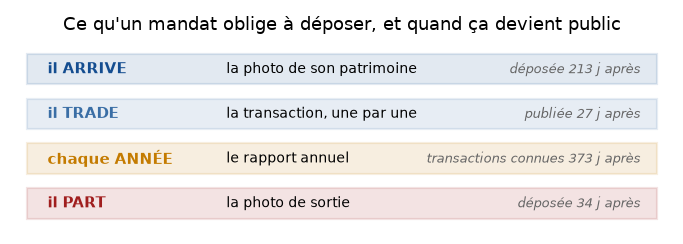
\includegraphics[width=0.74\textwidth]{fig_10_obligations.png}\\[2mm]
  \defl{médianes mesurées sur nos dépôts, pas des délais légaux recopiés --- et elles ne partent pas
  du même repère : \textbf{213 j après l'entrée en fonction} (n = 258) · \textbf{27 j} et
  \textbf{373 j après l'opération} (q90 49 et 540 j) · \textbf{34 j après la fin du mandat}
  (n = 374).}\\[2mm]
  \piege{le rapport annuel n'est pas une redite tardive sans intérêt : c'est le seul canal qui
  voit 103 des 408 membres qui tradent. Mais son information a plus d'un an quand elle devient publique.}
\end{frame}

% ── 1 · IL ARRIVE ───────────────────────────────────────────────────────────────
\pipeslide{1}{1 · Il arrive}
  {que possède un élu au moment où il entre en fonction ?}
  {319 des 461 arrivants déposent leur photo --- 325 photos d'entrée en main}

\begin{frame}{À l'arrivée : 319 des 461 arrivants déposent leur photo}
  \centering
  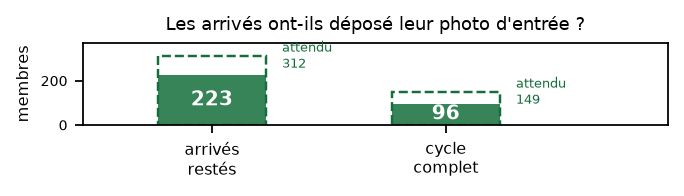
\includegraphics[width=0.60\textwidth]{fig_10_etape_arrivee.png}\\[1mm]
  \begin{columns}[t]
    \begin{column}{0.52\textwidth}\footnotesize
      \textbf{D'où sortent les 325 photos}\\[0.8mm]
      \begin{tabular}{@{}rl@{}}
        \textbf{378} & documents d'entrée \emph{H} au corpus\\
        \textbf{7\,670} & candidatures \emph{C} au corpus\\
        \textbf{291} & membres re-sélectionnés (dont 52 par un \emph{C})\\
        \textbf{+34} & gardés de la sélection précédente\\
        \midrule
        \textbf{325} & photos d'entrée retenues, une par membre\\
      \end{tabular}\\[1mm]
      \defl{la règle : le \emph{H} s'il existe, sinon le \emph{C} le plus proche du début de
      mandat, cherché dans les deux sources (électronique et scanné océrisé, acte II étape 5) ;
      les 34 photos que seule la sélection précédente retrouve sont conservées.}
    \end{column}
    \begin{column}{0.44\textwidth}\footnotesize
      \textbf{Attendu contre observé}\\[0.8mm]
      \begin{tabular}{@{}rl@{}}
        \textbf{461} & membres devaient en déposer une\\
        \textbf{319} & l'ont fait \; \textrightarrow{} \; \textbf{142} manquantes\\
        \textbf{+6} & photos chez des non-attendus\\
        \midrule
        \textbf{325} & photos d'entrée en main\\
      \end{tabular}\\[1.2mm]
      \defl{461 attendues = 312 arrivés restés + 149 cycles complets.}\\[2mm]
      \kpi{warnorange}{213 jours}{de délai médian entre l'entrée en mandat et le dépôt ---
      n = 258, les photos dont on connaît les deux dates}
    \end{column}
  \end{columns}
\end{frame}

\begin{frame}{Des 325 photos retenues, 261 portent au moins une action cotée}
  \footnotesize
  \begin{center}
  \begin{tabular}{@{}lrrl@{}}
    \toprule
    \textbf{Ce que contient la photo d'entrée} & \textbf{lignes} & \textbf{valeur} & \\
    \midrule
    actions et ETF cotés (négociables) & 11\,480 & 595 M\$ & \badgel{okgreen!25}{entre au moteur}\\
    fonds mutuels                      &  1\,726 & 219 M\$ & écarté par nature\\
    faux tickers (codes du formulaire) &     56 &   2 M\$ & écarté par nature\\
    monétaires                         &     48 &   1 M\$ & écarté par nature\\
    \midrule
    \textbf{total tickérisé}           & \textbf{13\,310} & \textbf{817 M\$} & \\
    \bottomrule
  \end{tabular}
  \end{center}
  \vspace{1mm}
  \begin{columns}[t]
    \begin{column}{0.52\textwidth}
      \textbf{La cascade des membres}\\[0.8mm]
      \begin{tabular}{@{}rl@{}}
        \textbf{325} & membres ont une photo retenue\\
        \textbf{288} & ont au moins une ligne tickérisée\\
        \textbf{261} & ont au moins une ligne négociable\\
        \textbf{172} & \emph{et} tradent : leur photo peut servir de départ\\
      \end{tabular}
    \end{column}
    \begin{column}{0.44\textwidth}
      \kpi{helec}{8\,860}{lignes (membre, ticker) après agrégation}\\[1.5mm]
      \defl{les 11\,480 lignes négociables se regroupent en 8\,860 couples (membre, ticker) :
      un même titre peut être déclaré sur plusieurs comptes.}
    \end{column}
  \end{columns}\vspace{2mm}\par
  \defl{le tableau ne couvre que les lignes \emph{tickérisées} de ces 325 photos : une photo porte
  aussi des lignes qu'aucun symbole ne désigne (immobilier, parts de société, comptes) --- le
  paysage complet est en acte II. \; « négociable / fonds / monétaire / faux ticker » : la classe
  est posée avant toute tickérisation, le détail de cette décision est en partie III.}
\end{frame}

% ── 2 · IL TRADE ────────────────────────────────────────────────────────────────
\pipeslide{2}{2 · Il trade}
  {qu'a-t-il acheté ou vendu, et quand l'apprend-on ?}
  {122\,814 lignes de transactions pour la Chambre, publiées 27 jours après l'opération}

\begin{frame}{La déclaration rapide est le seul document exploité à 100 \%}
  \footnotesize
  \begin{columns}[t]
    \begin{column}{0.50\textwidth}
      \textbf{Ce que le canal rapide apporte}\\[1.2mm]
      \begin{tabular}{@{}rl@{}}
        \textbf{5\,571} & dépôts (membre × date de divulgation)\\
        \textbf{122\,814} & lignes de transactions, Chambre\\
        \textbf{122\,809} & dans la fenêtre 2013-2026 ($-5$)\\
        \textbf{315} & membres concernés\\
        \textbf{4\,340} & tickers distincts\\
      \end{tabular}\\[2mm]
      \defl{les 122\,814 sont la part Chambre de la table de départ « clean » :
      134\,464 lignes = 122\,814 Chambre + 11\,650 Sénat.}
    \end{column}
    \begin{column}{0.46\textwidth}
      \kpi{okgreen}{100 \%}{des 8\,267 documents \emph{P} du journal sont exploités}\\[1.5mm]
      \defl{aucun autre type de document n'atteint ce taux : les photos de patrimoine perdent
      de 25 à 60 \% de leurs documents (chiffres en partie IV).}\\[3mm]
      \kpi{warnorange}{27 jours}{de délai médian entre l'opération et sa publication (q90 : 49 jours)}
    \end{column}
  \end{columns}\vspace{3mm}\par
  \piege{trois comptes de « documents \emph{P} » coexistent, avec trois définitions :
  \textbf{8\,267} documents au journal de traitement · \textbf{5\,571} dépôts au sens
  (membre × date de divulgation) · \textbf{5\,784} documents dans la matrice document × section.
  Et deux comptes de \emph{lignes} : \textbf{122\,814} dans la table de collecte S1/S2 (ci-contre,
  c'est elle qui alimente le flux) · \textbf{56\,002} extraites du corpus de documents
  (réconciliation à la charnière A/B, en fin d'acte). Toujours dire lequel on compte.}
\end{frame}

% ── 3 · IL DÉCLARE ──────────────────────────────────────────────────────────────
\pipeslide{3}{3 · Il déclare}
  {chaque année, que redit-il de son patrimoine et de ses mouvements ?}
  {5\,702 rapports annuels attendus --- un membre sur deux couvre au moins 85 \% de ses années}

\begin{frame}{Le membre médian a 85 \% de ses années de mandat couvertes}
  \centering
  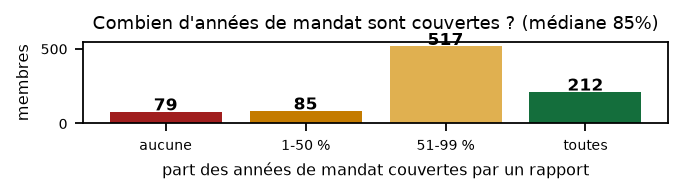
\includegraphics[width=0.50\textwidth]{fig_10_etape_annuel.png}\\[1mm]
  \begin{columns}[t]
    \begin{column}{0.50\textwidth}\footnotesize
      \textbf{Combien de rapports sont dus}\\[0.8mm]
      \begin{tabular}{@{}rl@{}}
        \textbf{5\,702} & rapports annuels attendus, 2013-2025\\
        \textbf{7} & membres n'en doivent aucun\\
        \textbf{893} & membres en doivent au moins un\\
        \textbf{814} & membres en ont déposé au moins un\\
      \end{tabular}\\[1mm]
      \defl{un rapport déposé en Y couvre Y$-$1 ; il est dû pour toute année en mandat au 31/12.
      La mesure porte sur \emph{chaque membre} : les 5\,702 années dues ne sont pas confrontées
      à un total observé.}
    \end{column}
    \begin{column}{0.46\textwidth}\footnotesize
      \textbf{Taux de couverture médian, par trajectoire}\\[0.8mm]
      \begin{tabular}{@{}lr@{}}
        cycle complet & 100 \%\\
        déjà-là restés & 92 \%\\
        arrivés restés & 86 \%\\
        déjà-là partis & 83 \%\\
        \midrule
        \textbf{médiane, 893 membres} & \textbf{85 \%}\\
      \end{tabular}\\[1mm]
      \defl{les barres de la figure comptent des \emph{membres}, pas des années.}
    \end{column}
  \end{columns}\vspace{1mm}\par
  \defl{ne pas trader n'est pas ne pas déclarer : sur les \textbf{509} membres que ni une déclaration
  rapide ni un rapport électronique ne montre en train de trader (492 + 17 du seul Schedule B
  océrisé), \textbf{444} (87 \%) déposent quand même des rapports.}
\end{frame}

% ── 4 · IL PART ─────────────────────────────────────────────────────────────────
\pipeslide{4}{4 · Il part}
  {que déclare-t-il en quittant la Chambre ?}
  {367 des 463 partants déposent leur photo, + 7 hors attendus --- un juge de fin de mandat}

\begin{frame}{À la sortie : 367 des 463 partants déposent, 96 manquent}
  \centering
  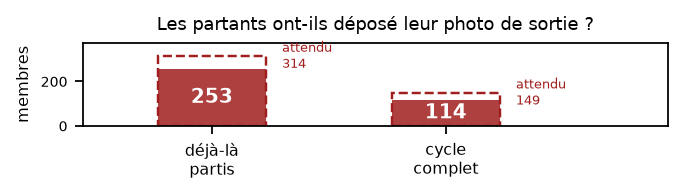
\includegraphics[width=0.64\textwidth]{fig_10_etape_sortie.png}\\[1mm]
  \begin{columns}[t]
    \begin{column}{0.50\textwidth}\footnotesize
      \textbf{Attendu contre observé}\\[0.8mm]
      \begin{tabular}{@{}rl@{}}
        \textbf{463} & membres devaient en déposer une\\
        \textbf{367} & l'ont fait \; \textrightarrow{} \; \textbf{96} manquantes\\
        \textbf{+7} & photos chez des membres restés\\
        \midrule
        \textbf{374} & membres avec photo de sortie\\
      \end{tabular}\\[1mm]
      \defl{463 attendues = 314 déjà-là partis + 149 cycles complets.}
    \end{column}
    \begin{column}{0.46\textwidth}\footnotesize
      \kpi{warnorange}{34 jours}{de délai médian entre la fin du mandat et le dépôt (n = 374)}\\[2.5mm]
      \textbf{La sortie porte aussi des mouvements}\\[0.8mm]
      \begin{tabular}{@{}rl@{}}
        \textbf{21\,175} & lignes de positions (379 documents)\\
        \textbf{9\,900} & lignes de transactions (157 documents)\\
      \end{tabular}\\[1mm]
      \defl{379 documents \emph{T} dans la table de positions, 378 dans l'inventaire des photos
      datées : deux tables, deux périmètres --- réconciliés deux slides plus loin.}
    \end{column}
  \end{columns}\vspace{1.5mm}\par
  \defl{la photo de sortie ne sert jamais à construire le portefeuille : elle est réservée
  au rôle de juge (acte II, étape 9).}
\end{frame}

% ── LA CHARNIÈRE A / B ──────────────────────────────────────────────────────────
\begin{frame}{Deux sections dans le formulaire, et elles ne servent pas à la même chose}
  \begin{columns}[c]
    \begin{column}{0.54\textwidth}
      \centering
      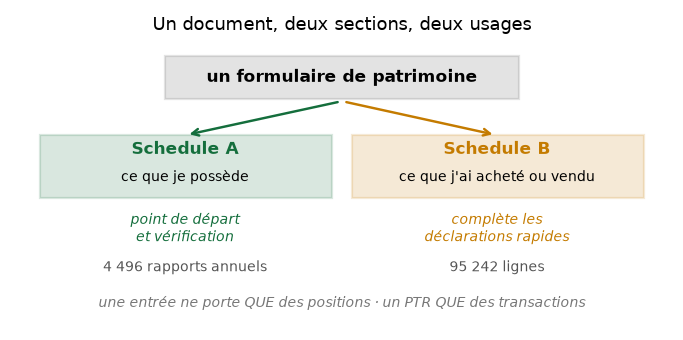
\includegraphics[width=\textwidth]{fig_10_deux_sections.png}\\[1mm]
      {\scriptsize\color{black!60} les deux chiffres portés sur la figure sont ceux du seul
      \emph{rapport annuel O} : 4\,496 documents de positions, 95\,242 lignes de transactions.
      Les totaux de section sont au tableau suivant.}
    \end{column}
    \begin{column}{0.44\textwidth}\footnotesize
      \textbf{\textcolor{okgreen}{Schedule A --- les positions}}\\
      ce qu'il \emph{possède}, à une date.\\
      \defl{donne le point de départ du portefeuille, et sert de juge à la fin.}\\[3mm]
      \textbf{\textcolor{warnorange}{Schedule B --- les transactions}}\\
      ce qu'il a \emph{acheté ou vendu}.\\
      \defl{fait bouger le portefeuille ; complète les déclarations rapides.}\\[3mm]
      \piege{« déclaration » ne dit rien : il faut toujours préciser \emph{quelle section}.
      La déclaration rapide \emph{P} ne porte que des transactions. L'entrée \emph{H} et la
      candidature \emph{C} ne portent que des positions. Le rapport annuel \emph{O}, l'amendement
      \emph{A} et la sortie \emph{T} portent les deux.}
    \end{column}
  \end{columns}
\end{frame}

\begin{frame}{Chaque type de dépôt ne porte que ce que le formulaire prévoit}
  \centering\scriptsize
  \begin{tabular}{@{}clrrrr@{}}
    \toprule
    & & \multicolumn{2}{c}{\textbf{POSITIONS} --- \emph{Schedule A}}
      & \multicolumn{2}{c}{\textbf{TRANSACTIONS}}\\
    \cmidrule(lr){3-4}\cmidrule(lr){5-6}
    code & document & documents & lignes & documents & lignes\\
    \midrule
    \emph{H} & entrée en fonction   &    378 &  22\,661 & \textbf{0} & \textbf{0}\\
    \emph{C} & candidature          & 7\,670 & 244\,759 & \textbf{0} & \textbf{0}\\
    \emph{O} & rapport annuel       & 4\,496 & 238\,624 & 2\,279 & 95\,242\\
    \emph{T} & sortie               &    379 &  21\,175 &    157 &  9\,900\\
    \emph{A} & amendement           & 1\,964 &  82\,667 &    314 &  5\,005\\
    \emph{P} & déclaration rapide   & \textbf{0} & \textbf{0} & 5\,784 & 56\,002\\
    \midrule
    & \textbf{total des positions} & \textbf{14\,887} & \textbf{609\,886} & & \\
    & \textbf{total \emph{Sch. B}} (\emph{O}+\emph{T}+\emph{A}) & & & & \textbf{110\,147}\\
    \bottomrule
  \end{tabular}\\[1mm]
  \defl{22\,661 + 244\,759 + 238\,624 + 21\,175 + 82\,667 = 609\,886 lignes sur 14\,887 documents
  (électronique + océrisé, acte II étape 5) \;·\; 95\,242 + 9\,900 + 5\,005 = 110\,147 lignes de
  Schedule B ; les 56\,002 lignes \emph{P}, elles, viennent du formulaire de déclaration rapide ---
  c'est l'objet de la slide suivante. L'amendement \emph{A} s'ajoute au dépôt qu'il corrige, sans
  le remplacer.}\\[0.4mm]
  \defl{ces comptes ne sont pas ceux de l'inventaire des photos datées (\emph{H} 376, \emph{C} 934,
  \emph{O} 4\,447, \emph{T} 378), qui ne garde que les documents datés et rattachés à un déposant.
  L'écart est massif sur \emph{C} : l'immense majorité des candidatures émane de candidats jamais
  élus, hors du registre. Seules 52 d'entre elles finissent en photo d'entrée.}\\[0.4mm]
  \piege{les trois cas à zéro (\emph{H} et \emph{C} côté transactions, \emph{P} côté positions) ne
  sont pas des trous d'extraction : ces formulaires ne comportent pas la section --- trois
  \co{assert} le contrôlent en non-régression, ils ne le démontrent pas.}
\end{frame}

\begin{frame}{76 \% du Schedule B est déjà dit par une déclaration rapide}
  \centering
  \vspace{2mm}
  \begin{tabular}{@{}rl@{}}
    \toprule
    \textbf{110\,147} & lignes de Schedule B \; \defl{(95\,242 \emph{O} + 9\,900 \emph{T} + 5\,005 \emph{A})}\\
    $-$ \textbf{84\,032} & déjà dites par une déclaration rapide \; \defl{(76 \% de redite)}\\
    \midrule
    = \textbf{26\,115} & transactions inédites --- le gisement réel des rapports\\
    \bottomrule
  \end{tabular}\\[4mm]
  \piege{deux comptes de lignes de déclarations rapides coexistent, et il faut dire lequel on
  compte : \textbf{56\,002} lignes extraites du corpus de documents --- c'est le compte à périmètre
  égal avec les 110\,147 ci-dessus --- et \textbf{122\,814} lignes dans la table de collecte
  S1/S2, plus complète, qui est la source réelle du flux construit à l'acte II.}\\[3mm]
  \choixbox{« déjà dite » est une règle, pas une évidence : une transaction du rapport est jugée
  connue si une déclaration rapide du même membre porte le même couple (titre, sens) à moins de
  \textbf{365 jours}. Cette seule constante décide du volume d'apport des rapports annuels ---
  aucune autre valeur n'a été mesurée (partie III).}
\end{frame}

% ── CE QUE L'ACTE I LAISSE ──────────────────────────────────────────────────────
\begin{frame}{Ce que l'acte I laisse entre nos mains}
  \scriptsize
  \begin{center}
  \begin{tabular}{@{}llr@{}}
    \toprule
    \textbf{Matière} & \textbf{Ce que c'est} & \textbf{Volume}\\
    \midrule
    Positions (Schedule A) & tout le Schedule A déposé, candidatures comprises & 609\,886 lignes\\
     & 5 types de documents sur 6 --- tout sauf la déclaration rapide \emph{P} & (14\,887 documents)\\
    \quad dont photos d'entrée & le point de départ, une par membre & 325 photos\\
    Transactions rapides (\emph{P}) & le fil de l'eau, Chambre --- table de collecte S1/S2 & 122\,814 lignes\\
     & \emph{le même canal, compté dans le corpus de dépôts} & \emph{56\,002 lignes}\\
    Transactions des rapports & Schedule B --- 110\,147 lignes, dont inédites & 26\,115 lignes\\
    \midrule
    Population & membres du registre & 900 membres\\
    \quad dont traders & au moins une transaction qu'on sait rejouer & 408 membres\\
    \bottomrule
  \end{tabular}
  \end{center}
  \vspace{2mm}
  \repband{le membre dépose \textbf{des documents}, pas des données : deux sections qui ne se
  mélangent jamais, des délais de 27 jours à plus d'un an, et des manques mesurés
  (142 photos d'entrée, 96 photos de sortie). Rien n'est encore trié, ni valorisé, ni reconstruit ---
  c'est l'objet de l'acte II.}
\end{frame}

% ═══════════ part2 ═══════════
% ══════════════════════════════════════════════════════════════════════════════
%  PART 2 — ACTE II (1) : 5 on rassemble · 6 on trie · 7 on valorise
% ══════════════════════════════════════════════════════════════════════════════

\partdivider{okgreen}{ACTE II}{Ce qu'on en fait}{de la ligne déclarée au portefeuille}

% ───────────────────────────────── ÉTAPE 5 ────────────────────────────────────
\pipeslide{5}{5 · On rassemble}
  {Combien de documents avons-nous ramassés, et que contient chacun d'eux ?}
  {6\,135 photos datées chez 887 déposants --- et 14\,887 documents portant 609\,886 lignes de positions}

\begin{frame}{Le corpus se compte d'abord en documents, ensuite en lignes}
  \centering
  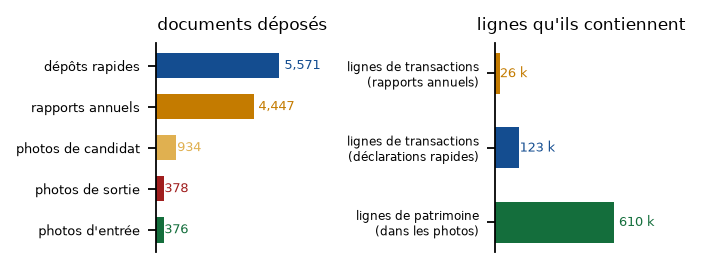
\includegraphics[trim={0 0 168bp 0},clip,width=0.31\textwidth]{fig_10_inventaire.png}\\[0.5mm]
  \defl{(les 139 amendements \emph{A} porteurs de flux net ne sont pas tracés)}\\[1mm]
  \begin{minipage}{0.96\textwidth}\footnotesize
  \textbf{Les documents de patrimoine} (une photo = un document daté) : 4\,447 rapports annuels
  \emph{O} + 934 photos de candidat \emph{C} + 378 photos de sortie \emph{T} + 376 photos d'entrée
  \emph{H} = \textbf{6\,135 documents}, chez 887 déposants \defl{(dont 12 candidats jamais élus)}.\\[0.8mm]
  \textbf{Le fil de l'eau}, à part : 5\,571 dépôts de déclaration rapide \emph{P} --- une paire
  (membre, date de divulgation) --- et 139 amendements \emph{A} porteurs de flux net.
  \end{minipage}\\[1mm]
  \defl{Deux unités jamais mélangées : le \textbf{document} et la \textbf{ligne}. Et deux
        dénombrements des mêmes dépôts, jamais additionnés : \textbf{6\,135} photos datées ici,
        \textbf{14\,887} documents porteurs d'au moins une ligne dans la table de positions.}
\end{frame}

\begin{frame}{L'océrisation était payée et n'était pas branchée : +188\,970 lignes}
  \footnotesize
  Les positions ne venaient que des dépôts \textbf{électroniques}. Les documents \textbf{scannés}
  avaient été passés à la reconnaissance de texte --- et la table des positions ne les voyait pas.
  \medskip

  \centering
  \begin{tabular}{l r r r}
    \toprule
    voie & documents & lignes & dont tickérisées \\
    \midrule
    dépôt électronique & 12\,459 & 420\,916 & 190\,758 \\
    document scanné, océrisé & 2\,428 & 188\,970 & \;\,81\,535 \\
    \midrule
    \textbf{table fusionnée} & \textbf{14\,887} & \textbf{609\,886} & \textbf{272\,293} \\
    \bottomrule
  \end{tabular}\\[1mm]
  \defl{tickérisée = un symbole boursier a pu être attaché au libellé de la ligne}
  \medskip

  \raggedright
  \choixbox{rattacher l'océrisation au patrimoine. Contrôles affichés avant de l'accepter :
    \textbf{0} document commun aux deux voies (assert) ; 43,2~\% des lignes océrisées sont
    tickérisées, contre 45,3~\% en électronique ; 124\,922 lignes sur 188\,970
    (\textbf{66,1~\%}) portent une fourchette conforme à la grille officielle ;
    et 20 lignes dont le symbole était en fait un code de formulaire sont neutralisées à la main.
    L'autre option (électronique seul) reste disponible, mais son effet global n'est pas re-mesuré.}
  \medskip

  \defl{La matrice « type de dépôt × section » posée en acte I vaut sur cette table fusionnée :
        609\,886 lignes de positions, et les transactions du \emph{Schedule B} comptées à part
        (110\,147 lignes, reprises à l'étape 7).}
\end{frame}

% ───────────────────────────────── ÉTAPE 6 ────────────────────────────────────
\pipeslide{6}{6 · On trie}
  {Cette ligne déclarée, est-ce une action cotée --- ou un fonds, un compte, un code de formulaire ?}
  {une classe par ligne, décidée avant tout prix ; seul le négociable entre au moteur}

\begin{frame}{On classe l'actif avant de connaître son prix}
  \footnotesize
  \textbf{La règle d'or} : chaque ligne reçoit sa classe à partir de son \emph{libellé},
  \emph{avant} toute recherche de prix. \textbf{Le moteur} --- le programme qui rejoue les opérations
  et tient le portefeuille de chaque membre (étape 8) --- ne voit ensuite que la classe
  \textbf{négociable} (action ou ETF coté).
  \medskip

  \centering
  Exemple sur les 26\,115 transactions de rapports annuels que les déclarations rapides
  n'avaient pas déjà dites :\\[1.5mm]
  \begin{tabular}{l r l}
    \toprule
    classe & lignes & décidée par \\
    \midrule
    négociable \defl{(action, ETF)} & 16\,062 & \defl{ticker reconnu, libellé d'actif} \\
    fonds mutuel                    & 9\,393  & \defl{ex. 5 lettres finissant par X} \\
    monétaire                       & 364    & \defl{7 codes listés (SPAXX, FDRXX, VMFXX\ldots)} \\
    faux ticker                     & 296    & \defl{19 codes de formulaire, 5 tickers ambigus bloqués} \\
    \midrule
    \textbf{total} & \textbf{26\,115} & \\
    \bottomrule
  \end{tabular}\\[2mm]

  \raggedright
  \piege{l'ancien moteur ne triait pas par classe, il gardait « ce qui a un prix ».
    Les trois classes écartées pèsent \textbf{9\,999} lignes (817~M\$) une fois retirés les
    221 échanges et les 14 dates hors fenêtre de l'étape 7 (290 faux tickers + 364 monétaires
    + 9\,345 fonds) --- et \textbf{7\,709} d'entre elles (486~M\$) avaient bel et bien une série de
    prix en cache (MEIIX 106 lignes, FXAIX 69, FHARX 55\ldots) : un fonds a une valeur liquidative,
    et il entrait donc dans le moteur \emph{actions}.}
\end{frame}

\begin{frame}{12\,790~M\$ d'actions et d'ETF sur 104\,130~M\$ déclarés}
  \footnotesize
  Le même classement, appliqué cette fois à \emph{toute} la table de positions : 609\,886 lignes,
  toutes années et tous types de dépôt confondus.
  \bigskip

  \centering
  \footnotesize
  \begin{tabular}{l r r}
    \toprule
    classe de la ligne & lignes & valeur déclarée \\
    \midrule
    sans aucun ticker \defl{(immobilier, LLC, notes, comptes)} & 337\,593 & 87\,405~M\$ \\
    négociable \defl{(action, ETF)}                            & 231\,426 & 12\,790~M\$ \\
    fonds mutuel                                               & 38\,885  & 3\,752~M\$ \\
    monétaire                                                  & 1\,106   & 99~M\$ \\
    faux ticker                                                & 876     & 84~M\$ \\
    \midrule
    \textbf{total déclaré} & \textbf{609\,886} & \textbf{104\,130~M\$} \\
    \bottomrule
  \end{tabular}\\[3mm]

  \raggedright
  \defl{12~\% de la valeur déclarée seulement passe le tri de l'étape 6. Les 337\,593 lignes sans
        aucun ticker --- immobilier, parts de sociétés, comptes, créances --- ne sont pas des
        erreurs : ce sont des actifs qu'aucun cours de bourse ne peut valoriser (leur tri est
        repris en partie IV).}
\end{frame}

\begin{frame}{Le « patrimoine » total empile treize ans de déclarations}
  \footnotesize
  \begin{columns}[T]
    \begin{column}{0.48\textwidth}
      \centering
      \colorbox{alertred!8}{\parbox{\dimexpr\linewidth-8pt}{\centering\vspace{1mm}
        \textbf{\textcolor{alertred}{Ce qu'on ne doit PAS appeler « le patrimoine »}}\\[1.5mm]
        {\Large\textbf{104\,130~M\$}}\\[0.8mm]
        609\,886 lignes\\[0.8mm]
        \defl{toutes les lignes déposées de 2014 à 2026, additionnées}\vspace{1mm}}}
    \end{column}
    \begin{column}{0.48\textwidth}
      \centering
      \colorbox{okgreen!10}{\parbox{\dimexpr\linewidth-8pt}{\centering\vspace{1mm}
        \textbf{\textcolor{okgreen}{Le stock, à une date}}\\[1.5mm]
        {\Large\textbf{8\,887~M\$}}\\[0.8mm]
        42\,522 lignes, 887 déposants\\[0.8mm]
        \defl{le dernier document de chaque membre, et lui seul}\vspace{1mm}}}
    \end{column}
  \end{columns}
  \medskip
  \centering \kpi{alertred}{12×}{d'écart entre les deux chiffres}\\[1mm]
  \defl{les \emph{dépôts} courent de 2014 à 2026 ; les \emph{dates d'opération}, elles, remontent
        à 2013 --- c'est la fenêtre des entonnoirs de l'étape 7}\\[2mm]

  \raggedright
  \piege{le même actif est \textbf{recompté à chaque rapport annuel}. Un membre qui détient
    la même action pendant dix ans la déclare dix fois : la somme de toutes les lignes déposées
    n'est pas un patrimoine, c'est un cumul de déclarations. Le seul chiffre qui répond à
    « combien possèdent-ils ? » est celui de droite --- et encore, à des dates différentes selon les membres.}
\end{frame}

\begin{frame}{Le libellé nomme souvent le compte, pas l'actif}
  \footnotesize
  Une ligne déclarée s'écrit fréquemment \co{Fidelity Rollover IRA $\Rightarrow$ Apple Inc.} :
  le \emph{compte} d'abord, l'\emph{actif} ensuite. Un test de classement qui lit le libellé
  entier voit « Fidelity » et classe la ligne en \textbf{fonds}.
  \medskip

  \choixbox{le test « est-ce un fonds ? » ne lit que ce qui suit la dernière flèche ---
    l'actif --- et non le libellé entier.}
  \medskip

  \centering
  \begin{tabular}{c c c}
    \colorbox{alertred!8}{\parbox{0.36\textwidth}{\centering\vspace{0.8mm}
      \scriptsize\textbf{\textcolor{alertred}{hier --- libellé entier}}\\[0.8mm]
      \co{Fidelity Rollover IRA} \\ \co{$\Rightarrow$ Apple Inc.}\\[0.8mm]
      classée \textbf{fonds}, hors moteur\vspace{0.8mm}}}
    & \Large$\rightarrow$ &
    \colorbox{okgreen!10}{\parbox{0.36\textwidth}{\centering\vspace{0.8mm}
      \scriptsize\textbf{\textcolor{okgreen}{aujourd'hui --- après la flèche}}\\[0.8mm]
      \co{Apple Inc.}\\[0.8mm]
      classée \textbf{négociable}, au moteur\vspace{0.8mm}}}
  \end{tabular}\\[3mm]

  \kpi{okgreen}{1\,211}{lignes rendues au moteur} \hspace{12mm}
  \kpi{okgreen}{460~M\$}{qu'elles représentent}\\[2mm]
  \defl{sur les 272\,293 lignes de patrimoine tickérisées ---
        les plus touchés : TF 26 lignes · AAPL 26 · VTI 19 · MSFT 18 · SPY 18 · FB 16}\\[3mm]

  \raggedright
  \defl{Des actions et des ETF parfaitement cotés étaient écartés du moteur à cause du nom
        de la maison de courtage qui les héberge. Le défaut est corrigé ; il dit surtout que
        la classe d'un actif se lit sur une chaîne de caractères, et qu'une chaîne peut mentir.}
\end{frame}

% ───────────────────────────────── ÉTAPE 7 ────────────────────────────────────
\pipeslide{7}{7 · On valorise}
  {Que reste-t-il quand on exige un cours de marché à la date de l'opération ?}
  {129\,538 transactions exploitables, venues de trois sources}

\begin{frame}{Le fil de l'eau : 122\,814 lignes déclarées, 107\,976 valorisables}
  \footnotesize
  Valoriser, c'est deux gestes : le montant déclaré est une \textbf{fourchette}, on en retient le
  \textbf{milieu} ; et la ligne doit avoir un \textbf{cours} à la date de l'opération. Les entonnoirs
  qui suivent comptent le second. Le départ, ici, est la table de transactions \textbf{nettoyée} livrée par la collecte (partie I) :
  122\,814 lignes pour la Chambre, la plus complète des deux extractions des déclarations rapides.
  \medskip

  \centering\scriptsize
  \begin{tabular}{l r r l}
    \toprule
    filtre & retiré & il reste & pourquoi \\
    \midrule
    départ --- déclarations rapides, Chambre & --- & 122\,814 & \defl{la table nettoyée de la partie I} \\
    date hors fenêtre 2013-2026        & $-$5      & 122\,809 & \defl{315 membres, 4\,340 tickers} \\
    aucune série de cours pour le ticker & $-$14\,833 & 107\,976 & \defl{305 membres : 10 membres perdus ici} \\
    opérations « exchange »            & $-$0      & 107\,976 & \defl{ni achat ni vente : aucune ici} \\
    \midrule
    \textbf{trades exploitables} & & \textbf{107\,976} & \\
    \bottomrule
  \end{tabular}\\[3mm]

  \raggedright\footnotesize
  \textbf{D'où vient le trou de 14\,833 lignes ?} L'univers des tickers négociables compte
  5\,468 symboles : \textbf{3\,192} séries déjà téléchargées et jamais modifiées $+$ \textbf{821}
  téléchargées pour ce travail $=$ \textbf{4\,013} disponibles, moins \textbf{80} exclues par le
  garde-fou de qualité (moins de 2 points, cours sous 0,10~\$, ou saut quotidien supérieur à
  300~\%) $=$ \textbf{3\,933} séries chargées ; les \textbf{1\,455} derniers symboles sont des échecs
  de téléchargement. Côté déclarations de la Chambre, \textbf{1\,234} symboles finissent sans aucun
  cours (1\,177 échecs confirmés au re-jeu du 22/07 $+$ 57 écartés par le garde-fou) --- ce sont eux qui emportent
  les lignes perdues : MMC 208 lignes, FI 200, WBA 190 en tête.
\end{frame}

\begin{frame}{Des 26\,115 transactions inédites, 14\,084 arrivent au moteur}
  \footnotesize
  Les \textbf{26\,115} transactions inédites des rapports annuels --- celles que les déclarations
  rapides n'avaient pas déjà dites --- ont été isolées en acte I. Voici ce qu'il en reste une fois
  exigés un sens, une date, une classe négociable et un cours.
  \medskip

  \centering\scriptsize
  \begin{tabular}{l r r l}
    \toprule
    filtre & retiré & il reste & pourquoi \\
    \midrule
    départ --- transactions inédites des rapports & --- & 26\,115 & \defl{isolées en acte I} \\
    opérations « exchange »        & $-$221   & 25\,894 & \defl{pas de sens directionnel} \\
    date hors fenêtre 2013-2026    & $-$14    & 25\,880 & \\
    aucun montant déclaré          & $-$0     & 25\,880 & \\
    faux tickers                   & $-$290   &        & \defl{codes de formulaire} \\
    monétaires                     & $-$364   &        & \defl{écartés par leur classe} \\
    fonds mutuels                  & $-$9\,345 & 15\,881 & \defl{la plus grosse perte} \\
    séries de cours corrompues     & $-$43    &        & \defl{garde-fou de qualité} \\
    aucune série de cours          & $-$1\,275 & 14\,563 & \defl{dont 700 libellés de compte} \\
    déjà dit par une déclaration rapide & $-$479 & 14\,084 & \defl{488 appariements exacts, 479 lignes retirées} \\
    \midrule
    \textbf{trades retenus} & & \textbf{14\,084} & \\
    \bottomrule
  \end{tabular}\\[2mm]

  \raggedright\footnotesize
  Chaque ligne écartée a une raison et \emph{une seule} : un assert vérifie que la cascade
  retombe exactement sur le nombre de trades effectivement injectés.
\end{frame}

\begin{frame}{Le Schedule B scanné : 155\,306 lignes brutes, 7\,478 neuves}
  \centering\scriptsize
  \begin{tabular}{l r r l}
    \toprule
    filtre & retiré & il reste & pourquoi \\
    \midrule
    départ --- Schedule B des documents océrisés & --- & 155\,306 & \defl{669 documents, 165 membres} \\
    sens illisible ou échange       & $-$3\,017  & 152\,289 & \defl{ni achat ni vente} \\
    aucun symbole reconnu           & $-$89\,337 & 62\,952  & \defl{on ne devine pas un ticker absent} \\
    ni action ni ETF                & $-$205    & 62\,747  & \defl{écartées par leur classe} \\
    date hors fenêtre 2013-2026     & $-$1\,550  & 61\,197  & \\
    aucun cours disponible          & $-$9\,338  & 51\,859  & \defl{candidates} \\
    document non rattaché à un membre & $-$1\,471 & 50\,388 & \defl{on ne sait pas à qui l'attribuer} \\
    déjà dit par une déclaration rapide \defl{(±365 j)} & $-$40\,807 & 9\,581 & \defl{la règle d'écho de l'acte I} \\
    doublons (membre, ticker, sens, date) & $-$2\,103 & 7\,478 & \defl{on garde le dépôt le plus ancien} \\
    \midrule
    \textbf{transactions ajoutées} & & \textbf{7\,478} & \defl{chez 57 membres} \\
    \bottomrule
  \end{tabular}\\[1mm]
  \defl{155\,306 $-$ 3\,017 $-$ 89\,337 $-$ 205 $-$ 1\,550 $-$ 9\,338 $-$ 1\,471 $-$ 40\,807 $-$ 2\,103 = 7\,478}\\[2mm]

  \raggedright
  \choixbox{ces documents ne portent pas de fourchette de montant exploitable :
    les 7\,478 transactions reçoivent toutes le même \textbf{forfait de 8\,000,5~\$}
    (milieu de la fourchette la plus fréquente). Le notebook le dit explicitement --- c'est un choix,
    et il borne la précision ; l'effet d'un autre forfait n'est pas mesuré.}
\end{frame}

\begin{frame}{Le flux final F : 129\,538 transactions, trois sources}
  \begin{columns}[T]
    \begin{column}{0.52\textwidth}
      \centering\scriptsize
      \begin{tabular}{l r}
        \toprule
        source & trades \\
        \midrule
        déclarations rapides \emph{P} & 107\,976 \\
        \defl{au fil de l'eau} & \\
        rapports annuels, voie électronique & 14\,084 \\
        \defl{11~\% du flux} & \\
        rapports annuels, Schedule B océrisé & 7\,478 \\
        \defl{chez 57 membres} & \\
        \midrule
        \textbf{flux unifié F} & \textbf{129\,538} \\
        \defl{chez 408 membres} & \\
        \bottomrule
      \end{tabular}
    \end{column}
    \begin{column}{0.46\textwidth}
      \footnotesize
      \textbf{Les trois sources ne pèsent pas au même moment.}\\[1.5mm]
      \scriptsize
      En \textbf{2014}, le scanné apporte \textbf{1\,657} trades (783 achats, 874 ventes),
      contre 731 pour les rapports électroniques (392 / 339) et 6\,343 pour les déclarations
      rapides (3\,563 / 2\,780).\\[1.5mm]
      En \textbf{2025}, le scanné ne pèse plus que \textbf{13} trades (12 / 1), contre 11\,526
      pour les déclarations rapides (5\,487 / 6\,039).\\[1.5mm]
      \defl{Le troisième canal ne sert donc presque qu'aux premières années --- celles où le
            dépôt papier était encore la norme.}
    \end{column}
  \end{columns}
  \vspace{2mm}

  \raggedright
  \repband{F = 129\,538 transactions chez 408 membres = 107\,976 (fil de l'eau) + 14\,084
    (rapports annuels électroniques) + 7\,478 (Schedule B océrisé). Les rapports annuels au sens
    large pèsent donc 21\,562 trades, soit 16,6~\% du flux. Avant l'union, 479 lignes ont été
    retirées (488 appariements exacts membre × ticker × sens × date), soit 3,4~\% des
    14\,563 transactions de rapports candidates.}
\end{frame}

% ═══════════ part3 ═══════════
% ══════════════════════════════════════════════════════════════════════════════
%  PART 3 — ACTE II (2) : 8 on reconstruit · 9 on vérifie
%  Source unique des chiffres : Portefeuilles_House_Complet.ipynb (cellules citées en commentaire).
% ══════════════════════════════════════════════════════════════════════════════

\pipeslide{8}{8 · On reconstruit}
  {Une photo datée, puis des transactions une à une : que détenait chaque membre, chaque jour ?}
  {376 portefeuilles quotidiens avec le dossier complet --- déclarations rapides $+$ photo d'entrée $+$ transactions des rapports annuels ---, dont 166 partis d'une photo réelle}

% ── 8.1 le principe (cell 79 MD, cell 88 code) ────────────────────────────────
\begin{frame}{Un portefeuille reconstruit compte des \emph{parts}, pas des dollars}
  \centering
  \bmaths{point de départ — la valeur déclarée, divisée par le prix du jour du dépôt}
         {h_{0,i} \;=\; \tilde v_i \,/\, P_i\!\left(\tau(f_0)\right)}
  \bmaths{achat — le montant déclaré achète des parts au prix du jour de l'opération}
         {h_i \;\mathrel{+}=\; q_i, \qquad q_i \;=\; \tilde v \,/\, P_i(\tau(t))}
  \bmaths{vente — on ne peut vendre que ce qu'on détient}
         {h_i \;\mathrel{-}=\; \min(q_i,\,h_i)}
  \defl{$i$ = un titre · $\tilde v$ = milieu de la fourchette déclarée · $P_i$ = cours de clôture du
  titre $i$ · $q_i$ = les parts que le montant déclaré représente au prix du jour}\\[0.5mm]
  \defl{$\tau(d)$ = premier jour coté $\geq d$ · $f_0$ = date de \textbf{dépôt} de la photo ·
  $t$ = date de l'\textbf{opération} déclarée}\\[4mm]
  \piege{Compter en parts n'est pas une coquetterie : le rendement du jour se calcule sur les parts
  de la \textbf{veille} (page suivante). Un apport --- la photo, ou un achat --- ne crée donc jamais
  de performance : c'est mesuré à l'étape 9.}
\end{frame}

% ── 8.1bis valeur et rendement (cell 88 code : daily_return) ──────────────────
\begin{frame}{Ce que vaut ce compte de parts, et ce qu'il rapporte}
  \centering
  \bmaths{valeur du jour — les parts détenues, au cours du jour}
         {V(\tau) \;=\; \textstyle\sum_i h_i(\tau)\,P_i(\tau)}
  \bmaths{rendement du jour — sur les parts de la veille, jamais sur celles du jour}
         {r(\tau) \;=\; \frac{\sum_i h_i(\tau-1)\,P_i(\tau)}{\sum_i h_i(\tau-1)\,P_i(\tau-1)} \;-\; 1}
  \defl{$\tau$ = un jour coté · la somme porte sur tous les titres détenus ce jour-là}\\[3mm]
  {\footnotesize C'est cette suite de rendements quotidiens, un nombre par membre et par jour de
  bourse, qui constitue \textbf{le portefeuille reconstruit}. Tout le reste du travail --- la
  vérification de l'étape 9, puis les tests --- se lit sur elle.}\\[3.5mm]
  \raggedright
  \choixbox{le rendement quotidien est écrêté à $\pm$50~\%, garde-fou contre les séries de cours
  aberrantes. Combien de jours-membres sont effectivement écrêtés, et ce que donnerait une autre
  borne, n'est \textbf{pas mesuré}.}
\end{frame}

% ── 8.2 le cas réel (cell 82) ─────────────────────────────────────────────────
\begin{frame}{Le cas réel : une fourchette déclarée devient 606,59 parts}
  \centering\small
  \begin{tabular}{llrrlrr}
    \toprule
    membre & titre & fourchette déclarée & milieu $\tilde v$ & date de dépôt & prix $P$ & parts $h_0$\\
    \midrule
    Jake Auchincloss & DMXF & 1\,001 -- 15\,000 \$ & 8\,000,5 \$ & 2021-07-29 & 59,6050 \$ & 134,23\\
    Richard W. Allen & BAC  & 1\,001 -- 15\,000 \$ & 8\,000,5 \$ & 2015-05-22 & 13,1892 \$ & 606,59\\
    \bottomrule
  \end{tabular}\\[3mm]
  \defl{les deux lignes tombent dans la même tranche : 1\,001 -- 15\,000 \$ est la fourchette la plus
  fréquente des déclarations · le prix est affiché à 4 décimales pour que la division tombe juste}\\[5mm]
  \kpi{okgreen}{8\,000,5 \$}{$\div$ 13,1892 \$} \kpi{okgreen}{$=$ 606,59 parts}{de Bank of America, le 22 mai 2015}\\[5mm]
  {\footnotesize Tout montant du dossier suit ce chemin, et lui seul : \textbf{fourchette déclarée
  $\rightarrow$ milieu $\rightarrow$ parts, au prix du jour}. Le portefeuille ne stocke jamais de
  dollars : il stocke 606,59 parts, qui vaudront ce que vaudra le titre.}\\[5mm]
  \repband{Ces deux quantités sont recalculées à la main, hors du moteur, et lui sont égales à
  $10^{-12}$ près --- avec la date : le premier jour coté retenu est bien le jour du dépôt.}
\end{frame}

% ── 8.3 photo fait foi (cells 87, 94, 65, 80) ─────────────────────────────────
\begin{frame}{La photo fait foi : 11\,277 trades ne sont plus rejoués}
  \small
  Une photo d'entrée déclare l'état \textbf{complet} du patrimoine à sa date. Rejouer un achat
  \emph{antérieur} à cette date ajouterait une seconde fois une position que la photo contient
  déjà : le même titre serait compté deux fois.\\[2mm]
  \centering
  \kpi{alertred}{11\,277}{trades écartés} \quad
  \kpi{alertred}{697 M\$}{de milieux de fourchette ($\tilde v$)} \quad
  \kpi{alertred}{88}{membres concernés}\\[2mm]
  \defl{les deux plus gros contributeurs : Daniel Goldman (1\,843 trades, 50,7 M\$) et Diana
  Harshbarger (1\,680 trades, 233,7 M\$)}\\[3mm]
  \raggedright
  \choixbox{\co{PHOTO\_FAIT\_FOI = True}. L'autre option (\co{False}) est l'ancien comportement du
  moteur : ces 11\,277 trades étaient rejoués \emph{en plus} de la photo, donc comptés deux fois.
  La règle suppose la photo \textbf{exhaustive à sa date} ; cette exhaustivité n'est pas vérifiée
  trade par trade.}\\[1.5mm]
  \piege{\og{}Sa date\fg{} est la date de \textbf{dépôt} du document, pas la date d'effet du
  patrimoine qu'il décrit : la photo d'entrée arrive en médiane \textbf{213 jours} après l'entrée en
  mandat (n = 258 photos d'entrée, une par membre). Le point de départ est donc jouable, mais tardif.}
\end{frame}

% ── 8.4 la cascade des photos (cells 83, 80 ; fig_10_entonnoir_h0) ────────────
\begin{frame}{De 325 photos d'entrée retenues à 166 portefeuilles injectés}
  \centering
  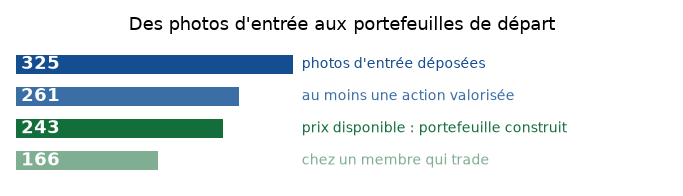
\includegraphics[width=0.78\textwidth]{fig_10_entonnoir_h0.png}\\[0.5mm]
  {\scriptsize
  325 \textbf{retenues}, une par membre (la figure dit \og{}déposées\fg{})
  $-$ \textbf{64} sans ligne négociable valorisée
  $=$ \textbf{261} portant au moins une action valorisée
  $-$ \textbf{18} sans prix au 1\up{er} jour coté $=$ \textbf{243} initialisables
  $=$ \textbf{166} injectées $+$ \textbf{77} sans trade à simuler}\\[1mm]
  \raggedright\scriptsize
  \textbf{Pourquoi on en perd à chaque marche.}
  \begin{itemize}\itemsep0pt\parskip0pt
    \item les \textbf{64} : la photo ne porte que du non coté, des fonds ou des libellés de compte --- rien à valoriser en actions ;
    \item les \textbf{18} : le titre existe, mais aucune série de cours ne commence avant le jour du dépôt ;
    \item les \textbf{77} : le portefeuille de départ est construit, mais le membre n'a aucune transaction à lui appliquer.
  \end{itemize}
  \vspace{0.5mm}
  \centering
  \kpi{okgreen}{7\,782}{lignes (membre, ticker) converties en parts} \quad
  \kpi{okgreen}{84,5 \%}{de la valeur \emph{négociable} des photos (595 M\$)}\\[0.5mm]
  \defl{7\,782 des 8\,860 lignes (membre, ticker) négociables vues en partie I --- les 1\,080 autres
  n'ont pas de cours au jour du dépôt}
\end{frame}

% ── 8.5 partir de zéro (cells 46, 83, 93 ; fig_10_troncature) ─────────────────
\begin{frame}{166 membres partent d'une photo, 242 d'un portefeuille vide}
  \begin{columns}[T]
    \begin{column}{0.50\textwidth}
      \centering
      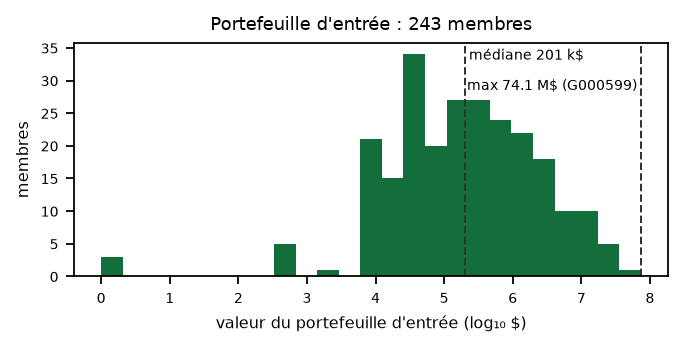
\includegraphics[width=\linewidth]{fig_10_h0_couverture.png}\\[0.5mm]
      \defl{les 243 portefeuilles de départ construits --- dont les 166 injectés\\
      médiane \textbf{201\,010~\$} · maximum \textbf{74\,104\,236~\$} (Daniel Goldman)}
    \end{column}
    \begin{column}{0.46\textwidth}
      \small
      Sur les \textbf{408} membres qui tradent :
      \begin{itemize}\itemsep2pt
        \item \textbf{172} ont déposé une photo d'entrée exploitable ;
        \item \textbf{166} d'entre eux ont un prix au premier jour coté : ce sont les
              \textbf{166 portefeuilles réellement injectés} ;
        \item les \textbf{242} autres démarrent d'un patrimoine \textbf{nul}.
      \end{itemize}
    \end{column}
  \end{columns}
  \vspace{2mm}
  \piege{Deux compteurs voisins. \textbf{236} $=$ 408 $-$ 172 $=$ les membres \emph{sans photo
  exploitable} ; \textbf{242} $=$ 408 $-$ 166 $=$ ceux qui \emph{démarrent vide} (les 236, plus les
  6 dont la photo n'a pas de prix).}
\end{frame}

% ── 8.6 les quatre reconstructions (cells 89-93) ──────────────────────────────
\begin{frame}{Quatre reconstructions, une seule mécanique}
  \centering\footnotesize
  \begin{tabular}{lrr}
    \toprule
    jeu de données & membres reconstruits & photos injectées\\
    \midrule
    A --- déclarations rapides seules                          & 226 & 0\\
    B --- déclarations rapides $+$ photo d'entrée              & 258 & 131\\
    C --- déclarations rapides $+$ rapports annuels (sans photo) & 355 & 0\\
    \textbf{D --- déclarations rapides $+$ photo $+$ rapports annuels} & \textbf{376} & \textbf{166}\\
    \bottomrule
  \end{tabular}\\[1.5mm]
  \defl{D est le \textbf{dossier complet}, la reconstruction retenue · chaque \og{}$+$\fg{} s'entend
  par rapport à A, jamais par rapport à la ligne du dessus : C ne contient aucune photo}\\[3mm]
  \raggedright\scriptsize
  \textbf{Décomposition des 166 photos de D} : les 131 déjà injectées en B, plus \textbf{35} membres
  que seuls les rapports annuels font apparaître dans le flux --- leur photo attendait un trade à
  simuler.\\[2mm]
  \piege{\og{}Membres\fg{} compte ici les membres dotés d'une \emph{série de rendement exploitable} :
  376 sur les 408 du flux. Un membre sort de la reconstruction si aucun de ses trades ne trouve de
  prix, si sa série tient en moins de deux jours, ou si elle ne bouge pas du tout.}
\end{frame}

% ── 8.7 la troncature des ventes (cells 89-93, 100 ; fig_10_troncature) ───────
\begin{frame}{Partir de zéro coûte 907 M\$ de ventes qu'on ne peut pas passer}
  \small
  Une vente déclarée peut ne trouver \textbf{aucune position en face} --- le membre a acheté le titre
  avant d'être observé. La règle $h_i \mathrel{-}= \min(q_i, h_i)$ ne vend alors que ce qui est
  détenu, et le surplus est journalisé en dollars au lieu d'être joué.\\[4mm]
  \centering\footnotesize
  \begin{tabular}{lr}
    \toprule
    reconstruction & ventes tronquées\\
    \midrule
    A --- déclarations rapides seules                                  & 937 M\$\\
    B --- déclarations rapides $+$ photo d'entrée                      & 688 M\$\\
    C --- déclarations rapides $+$ rapports annuels (sans photo)       & 1\,177 M\$\\
    \textbf{D --- dossier complet}                                     & \textbf{907 M\$}\\
    \bottomrule
  \end{tabular}\\[4mm]
  \raggedright\scriptsize
  Ajouter la photo d'entrée \textbf{réduit} la troncature de 27~\% (937 $\rightarrow$ 688 M\$) ;
  ajouter les rapports annuels l'\textbf{augmente} de 26~\% (937 $\rightarrow$ 1\,177 M\$) : cette
  reconstruction fait entrer 129 membres de plus (355 contre 226) et aucun d'eux ne part d'une photo.
  Le dossier complet, qui fait les deux, retombe à \textbf{907 M\$} --- soit 3~\% de moins que le
  témoin, pour 150 membres reconstruits de plus.
\end{frame}

\pipeslide{9}{9 · On vérifie}
  {La reconstruction est-elle juste --- et qui a le droit de le dire ?}
  {3\,435 confrontations avec des sections de positions qui n'ont jamais servi à construire : rappel médian 9 \% $\rightarrow$ 57 \%}

% ── 9.1 le principe (cells 88, 101 MD, 102, 109) ──────────────────────────────
\begin{frame}{Aucune position qui juge n'a servi à construire}
  \small
  \begin{columns}[T]
    \begin{column}{0.48\textwidth}
      \badge{okgreen}{CE QUI CONSTRUIT}\\[1.5mm]
      \begin{itemize}\itemsep2pt
        \item \textbf{une seule} photo de positions par membre : la photo d'\textbf{entrée} (H ou C) ;
        \item les \textbf{transactions} : déclarations rapides \textbf{P}, et Schedule B des
              rapports annuels \textbf{O}, des amendements \textbf{A} et des photos de sortie
              \textbf{T} --- en abrégé, O/A/T.
      \end{itemize}
    \end{column}
    \begin{column}{0.48\textwidth}
      \badge{helec}{CE QUI JUGE}\\[1.5mm]
      \begin{itemize}\itemsep2pt
        \item les \textbf{positions} déclarées dans les rapports annuels \textbf{O} (Schedule A) ;
        \item les \textbf{positions} de la photo de \textbf{sortie T}.
      \end{itemize}
    \end{column}
  \end{columns}
  \vspace{3mm}
  \centering
  \repband{Aucune position d'un rapport annuel ni d'une photo de sortie n'entre jamais dans le
  portefeuille. Le seul stock injecté est la photo d'entrée. C'est ce qui rend la mesure honnête :
  le juge n'a pas dicté sa réponse.}\\[2mm]
  \raggedright
  \piege{Un rapport annuel a \emph{deux} sections. Sa section \textbf{B} (transactions) nourrit le
  flux du dossier complet ; sa section \textbf{A} (positions) sert de juge. Les deux ne se
  recouvrent pas, mais elles viennent du même dépôt --- et il en va de même de la photo de sortie
  \textbf{T}, dont la section B alimente le flux quand sa section A sert de juge. Ce qui n'a jamais
  construit, ce sont les \emph{positions}, pas les documents.}
\end{frame}

% ── 9.2 le juge filtré (cells 102, 104) ───────────────────────────────────────
\begin{frame}{Le juge est lui aussi filtré : 2\,263 photos annuelles}
  \small
  Un rapport annuel ne peut juger que ce que le moteur prétend tenir : des actions et des ETF
  cotés, valorisés, dont on connaît le cours. Le juge subit donc le même tri que la reconstruction.\\[3mm]
  \centering
  \kpi{helec}{2\,263}{rapports exploitables (sur 4\,447)} \quad
  \kpi{helec}{460}{membres porteurs (le vivier)} \quad
  \kpi{helec}{43\,019}{lignes de positions}\\[2mm]
  \defl{les 2\,184 documents écartés ne portent aucune ligne négociable valorisée avec un cours ---
  le même tri que la reconstruction, marche par marche non chiffrée ici}\\[3mm]
  \begin{tabular}{lrl}
    \toprule
    on confronte & confrontations & lecture\\
    \midrule
    A (témoin) --- déclarations rapides seules & 1\,557 & le point de comparaison\\
    D (adaptée) --- dossier complet            & 1\,878 & la reconstruction retenue\\
    \midrule
    \textbf{total} & \textbf{3\,435} & \\
    \bottomrule
  \end{tabular}\\[1mm]
  \defl{une confrontation $=$ une photo O $\times$ une reconstruction}\\[2.5mm]
  \defl{460 est le vivier, pas le nombre de membres jugés : une photo n'est jugeable que si la
  reconstruction a bâti un portefeuille pour ce membre --- D en bâtit 376, A seulement 226.}
\end{frame}

% ── 9.3 les trois mesures (cells 104, 106 ; fig_10_recouvrement) ──────────────
\begin{frame}{Trois mesures, définies avant d'être chiffrées}
  \footnotesize
  À la date de dépôt de chaque rapport annuel, on compare deux ensembles de titres : ce que le
  document \textbf{déclare}, ce que le moteur \textbf{reconstruit}.
  \begin{itemize}\itemsep2pt
    \item \textbf{rappel} $=$ communes / déclarées --- \emph{ai-je retrouvé ce qu'il dit posséder ?}
    \item \textbf{précision} $=$ communes / reconstruites --- \emph{ce que je lui prête, le déclare-t-il ?}
    \item \textbf{fourchette} $=$ sur les seules positions communes, la valeur reconstruite $h \cdot P$
          tombe-t-elle entre les deux bornes déclarées ? (tolérance $\pm$0,1 \% sur les bornes)
  \end{itemize}
  \vspace{-2mm}
  \begin{center}
    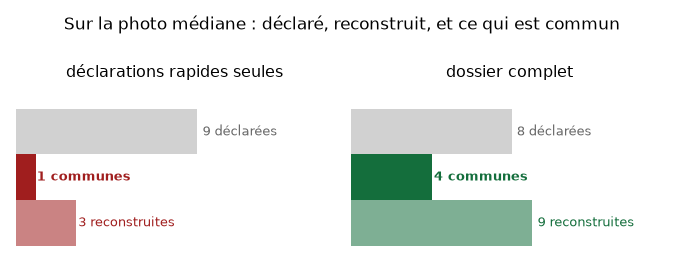
\includegraphics[width=0.58\textwidth]{fig_10_recouvrement.png}
  \end{center}
  \vspace{-5mm}
  \piege{Chaque panneau porte trois barres : des médianes prises \textbf{séparément}, colonne par
  colonne. Leur rapport n'est \textbf{pas} le rappel médian de la page suivante, qui est la médiane
  des rapports calculés photo par photo --- la médiane d'un quotient n'est pas le quotient des
  médianes.}
\end{frame}

% ── 9.4 le verdict (cell 105 ; fig_10_verif_dist) ─────────────────────────────
\begin{frame}{Le dossier complet fait passer le rappel médian de 9 \% à 57 \%}
  \centering
  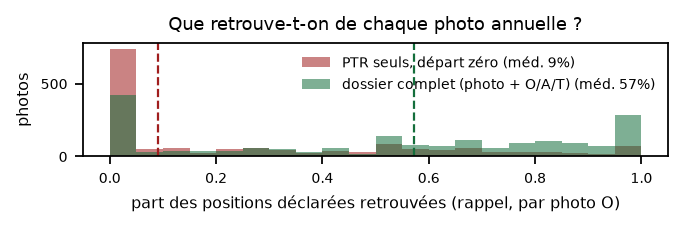
\includegraphics[width=0.62\textwidth]{fig_10_verif_dist.png}\\[0.5mm]
  \defl{sur la figure, O/A/T $=$ rapports annuels, amendements et photos de sortie}\\[1.5mm]
  \scriptsize
  \begin{tabular}{lrrl}
    \toprule
    mesure & A --- rapides seules & D --- dossier complet & \\
    \midrule
    rappel médian \emph{par photo}                & 9 \%  & \textbf{57 \%} & le saut\\
    précision médiane \emph{par photo}            & 55 \% & 56 \%          & voir ci-dessous\\
    valeurs en fourchette, \emph{part des positions communes} & 44 \% & 47 \% & à peine\\
    \bottomrule
  \end{tabular}\\[2mm]
  \raggedright
  \piege{(1) A et D ne sont pas jugés sur le \textbf{même jeu de photos} (1\,557 contre 1\,878) :
  une partie du saut vient des membres que A ne reconstruit pas du tout --- cet effet de composition
  n'est pas isolé. (2) La précision n'existe que si la reconstruction tient au moins une position ce
  jour-là : sa médiane laisse de côté les photos où A ne reconstruit rien, que le rappel, lui,
  compte à 0~\%.}
\end{frame}

% ── 9.5 la photo de sortie (cell 109) ─────────────────────────────────────────
\begin{frame}{Un second juge, d'un autre type de document : la photo de sortie}
  \small
  La photo de sortie \textbf{T} est déposée en fin de mandat et déclare le patrimoine à ce
  moment-là. Ses \textbf{positions} n'ont servi à rien dans la construction : elles offrent une
  réconciliation finale, sur un type de document différent des rapports annuels.\\[3mm]
  \piege{Comme pour les rapports annuels, ce sont ses \emph{positions} qui jugent : les
  transactions du Schedule B de ces mêmes photos de sortie, elles, nourrissent le flux (157
  documents, 9\,900 lignes, vus en partie I).}\\[4mm]
  \centering
  \kpi{helec}{136}{confrontations} \quad
  \kpi{okgreen}{60 \%}{rappel médian} \quad
  \kpi{okgreen}{55 \%}{précision médiane}\\[2mm]
  \defl{378 photos de sortie déposées ; 136 confrontations, dans la seule configuration D --- le
  dossier complet. Le nombre de photos T survivant au tri \og{}négociable, valorisé, avec prix\fg{}
  n'est pas chiffré ici : la perte entre 378 et 136 n'est donc pas décomposée.}\\[4mm]
  \raggedright
  \piege{L'échantillon est petit --- 136 confrontations contre 1\,878 pour les rapports annuels ---
  parce que peu de membres réunissent à la fois une photo de sortie exploitable et un portefeuille
  reconstruit. Un rappel un peu meilleur (60 \% contre 57 \%) ne se lit donc pas comme une
  progression : c'est un autre échantillon.}
\end{frame}

% ── 9.6 les recomptes à la main (cells 82, 96, 97, 98, 111) ───────────────────
\begin{frame}{Cinq recomptes à la main, chacun avec sa portée exacte}
  \centering\scriptsize
  \begin{tabular}{p{4.3cm}p{3.5cm}p{3.3cm}l}
    \toprule
    ce qui est recompté hors moteur & sur quoi & portée du test & écart toléré\\
    \midrule
    les parts initiales $h_0$ & 2 lignes (DMXF, BAC) & échantillon : 2 sur 7\,782 & $10^{-12}$\\
    les rendements quotidiens & Daniel Goldman, 869 rendements & exhaustif \emph{sur ce membre},
      reconstruction B & $10^{-9}$\\
    une photo de vérification & Kathy Castor, mai 2026 & 1 photo sur 1\,878 & $10^{-12}$\\
    un apport ne crée aucun rendement & photo seule, zéro trade & 1 cas construit exprès & $10^{-15}$\\
    B $\equiv$ A pour qui n'a pas de photo & reconstructions B et A & échantillon : 50 des 127
      membres de B sans photo injectée (258 $-$ 131) & égalité stricte\\
    \bottomrule
  \end{tabular}\\[3mm]
  \raggedright\footnotesize
  \textbf{Le recompte de la photo, en clair.} Kathy Castor, rapport déposé le 24 mai 2026 :
  \textbf{18} positions déclarées, \textbf{35} reconstruites, \textbf{16} communes
  $\rightarrow$ précision 16/35 $=$ \textbf{46 \%}, rappel 16/18 $=$ \textbf{89 \%} --- identiques à
  la table de vérification.\\[1.5mm]
  \textbf{Un apport n'est pas une performance.} Le jour de l'injection de la photo (2023-08-14),
  le rendement vaut \textbf{0} exactement ; dès le lendemain la position vit : $-$0,79 \%.
\end{frame}

% ── 9.7 les limites de la vérification (cells 105, 112 MD) ────────────────────
\begin{frame}{Ce que cette vérification ne prouve pas}
  \small
  \begin{itemize}\itemsep3pt
    \item elle ne juge que des \textbf{titres cotés} : tout ce que le membre déclare hors ticker
          (immobilier, parts de société, notes) est hors du jeu, des deux côtés ;
    \item la mesure de valeur est \textbf{indulgente par construction} : les fourchettes déclarées
          sont larges, et pourtant seules \textbf{47 \%} des positions communes y tombent ;
    \item la photo décrit le \textbf{31 décembre}, mais elle est confrontée au \textbf{jour du dépôt} :
          ce qui a bougé entre les deux dates compte contre la reconstruction ;
    \item les \textbf{amendements A} ne sont pas re-fusionnés aux rapports O qu'ils corrigent :
          limite déclarée, non chiffrée.
  \end{itemize}
  \vspace{2mm}
  \piege{Même dans la meilleure configuration, sur la photo médiane, \textbf{43 \%} des positions
  déclarées ne sont pas reconstruites et \textbf{44 \%} des positions reconstruites ne sont pas
  déclarées. Le dossier complet réduit l'écart ; il ne le ferme pas.}
\end{frame}

% ── 9.8 la réponse de l'acte II ───────────────────────────────────────────────
\begin{frame}{La reconstruction est mesurée, pas décrétée}
  \centering\vspace{2mm}
  \tuile{okgreen}{166}{portefeuilles partis\\ d'une photo réelle}
  \tuile{okgreen}{376}{membres reconstruits,\\ dossier complet}
  \tuile{helec}{3\,435}{confrontations\\ avec un juge}
  \tuile{helec}{57 \%}{rappel médian,\\ dossier complet}\\[6mm]
  \repband{Chaque portefeuille est un compte de parts : il part d'une photo datée quand elle existe
  --- 166 cas sur les 408 membres qui tradent --- et de zéro sinon. Il est jugé sur 1\,878
  confrontations tirées des 2\,263 rapports annuels exploitables, plus 136 photos de sortie : des
  \textbf{positions déclarées} qui n'entrent jamais dans le portefeuille. Il retrouve 57 \% des
  positions de la photo médiane, contre 9 \% avec les seules déclarations rapides, pour une
  précision de 56 \% et 47 \% de valeurs dans la fourchette. Cinq recomptes à la main confirment le
  calcul là où ils portent.}
\end{frame}

% ═══════════ part4 ═══════════
% ════════════════════════════════════════════════════════════════════════════════
%  PARTIE III — LES CHOIX
%  Cette partie n'est PAS une re-narration du trajet : chaque choix est raconté là où
%  il est né (actes I et II). On ne garde ici que les trois choix qui ne sont racontés
%  nulle part ailleurs, les trois défauts corrigés, et le tableau de TOUS les choix.
% ════════════════════════════════════════════════════════════════════════════════
\chapdivider{PARTIE III}{Les choix qu'on a faits}{chacun déplace des chiffres --- les voici}

% ── CHOIX — la fenêtre d'écho ────────────────────────────────────────────────────
\begin{frame}{Une fenêtre d'un an décide de l'apport des rapports}
  \vspace{0pt}
  {\footnotesize Le rapport annuel redit des transactions déjà déclarées au fil de l'eau.
   Règle retenue : une transaction d'un rapport est \textbf{déjà connue} si une déclaration
   rapide du même membre porte le même couple (titre, sens) à \textbf{365 jours ou moins,
   avant ou après} --- la fenêtre est bilatérale.}\par\vspace{1.5mm}
  \begin{center}\bmaths{constante du notebook}{\co{ECHO\_JOURS} = 365~\text{jours}}\end{center}
  \vspace{-3mm}
  \begin{center}{\footnotesize
  \begin{tabular}{lr}
    \toprule
    lignes du Schedule B (transactions des rapports) & 110\,147\\
    dont déjà dites par une déclaration rapide & $-$\,84\,032 \defl{(76 \%)}\\
    \midrule
    \textbf{transactions inédites retenues} & \textbf{26\,115}\\
    \bottomrule
  \end{tabular}}\end{center}
  \vspace{1mm}
  {\scriptsize Le test compare l'écart de dates $|$date du rapport $-$ date de la déclaration
   rapide$|$ au seuil : à fenêtre nulle, seules les redites portant \emph{exactement} la même
   date de transaction seraient détectées.}\par\vspace{1.5mm}
  \choixbox{la fenêtre est bilatérale : $\pm$365 jours autour de la transaction.
  \textbf{Aucune autre valeur n'a été mesurée} --- l'apport de 26\,115 lignes est à lire
  comme une \textbf{borne basse}, pas comme un résultat encadré : une fenêtre plus étroite
  déclarerait moins de redites, donc davantage de lignes inédites.}
\end{frame}

% ── CHOIX — la déduplication ─────────────────────────────────────────────────────
\begin{frame}{Même transaction, deux documents : le plus ancien gagne}
  \vspace{0pt}
  {\footnotesize La clé de doublon est la même partout :
   (\textbf{membre}, \textbf{titre}, \textbf{sens}, \textbf{date de transaction}).}\par\vspace{2mm}
  {\footnotesize\textbf{Deux applications, deux volumes}}\par\vspace{1mm}
  {\scriptsize
  \begin{tabular}{@{}>{\raggedright\arraybackslash}p{0.33\textwidth}r>{\raggedright\arraybackslash}p{0.42\textwidth}@{}}
    \toprule
    \textbf{où} & \textbf{lignes retirées} & \textbf{ce qui survit}\\
    \midrule
    à l'intérieur du gisement scanné
      & 2\,103 & le document déposé le plus tôt \defl{(9\,581 $\rightarrow$ 7\,478)}\\
    \addlinespace[0.6mm]
    entre sources : collision exacte avec nos propres déclarations rapides
      & \phantom{0}479 & la déclaration rapide, déposée en médiane 27 j après l'opération
        contre 373 j pour le rapport \defl{(14\,563 $\rightarrow$ 14\,084)}\\
    \bottomrule
  \end{tabular}}\par\vspace{2mm}
  {\scriptsize Ces \textbf{479} lignes distinctes sont retirées pour \textbf{488} appariements
   \defl{(3,35 \% du flux des rapports)} : plusieurs déclarations rapides peuvent s'apparier à
   une même ligne de rapport. Un test vérifie qu'il n'en reste aucune.}\par\vspace{2mm}
  \choixbox{conséquence directe et assumée : un \textbf{amendement} déposé après coup ne
  corrige jamais l'original --- il arrive plus tard, donc il perd. Dans la vérification, les
  amendements ne sont pas non plus re-fusionnés aux rapports annuels. L'autre option --- le
  dernier dépôt fait foi --- n'est \textbf{pas} mesurée.}
\end{frame}

% ── CHOIX — le gisement mesuré et non branché ────────────────────────────────────
\begin{frame}{Un gisement mesuré, chiffré, et laissé de côté}
  \centering
  {\footnotesize\textbf{Les déclarations rapides océrisées}}\\[1.5mm]
  \kpi{dataC}{105\,074}{lignes}\quad
  \kpi{dataC}{2\,337}{documents scannés}\\[2mm]
  \defl{dont ceux qui ne sont jamais arrivés par la voie électronique :}\\[1.5mm]
  \kpi{alertred}{879}{documents}\quad
  \kpi{alertred}{15\,381}{lignes}\quad
  \kpi{alertred}{124}{membres concernés}\\[3mm]
  \begin{minipage}{0.92\textwidth}{\footnotesize
   \textbf{Pourquoi on ne les branche pas :} sur ces 15\,381 lignes, \textbf{6\,238} ne portent
   aucun symbole résolu ; parmi les 9\,143 qui en portent un, \textbf{81 \%} --- 7\,441 lignes ---
   ont reçu leur symbole d'un \textbf{modèle de langage}, qui le devine à partir du libellé
   au lieu de le lire sur le document ; \textbf{1\,470} le tiennent d'un traitement antérieur, et
   \textbf{232} lignes seulement portent un symbole réellement imprimé sur le document.
   \defl{6\,238 $+$ 7\,441 $+$ 1\,470 $+$ 232 $=$ 15\,381.}}\end{minipage}\\[3mm]
  \choixbox{ces 15\,381 lignes sont mesurées puis \textbf{non injectées} : le flux final reste
  \textbf{129\,538} trades $=$ 107\,976 (déclarations rapides) $+$ 14\,084 (rapports
  électroniques) $+$ 7\,478 (Schedule B scanné). Les brancher ferait entrer des symboles
  devinés par une machine dans un signal d'achat --- leur apport n'est \textbf{pas} chiffré
  au-delà du volume ci-dessus.}
\end{frame}

% ── LES TROIS DÉFAUTS CORRIGÉS ───────────────────────────────────────────────────
\begin{frame}{Trois défauts corrigés : ce qu'ils valaient, ce qu'ils valent}
  \vspace{0pt}
  {\scriptsize
  \begin{tabular}{@{}>{\raggedright\arraybackslash}p{0.25\textwidth}>{\raggedright\arraybackslash}p{0.33\textwidth}>{\raggedright\arraybackslash}p{0.33\textwidth}@{}}
    \toprule
    \textbf{le défaut} & \textbf{avant} & \textbf{après}\\
    \midrule
    Le portefeuille d'entrée était compté \textbf{deux fois}
      & les trades antérieurs à la photo étaient rejoués \emph{par-dessus} la photo qui les
        déclare déjà
      & \textbf{11\,277} trades écartés, soit \textbf{697 M\$} de montants de transactions,
        chez \textbf{88} membres\\
    \addlinespace[0.6mm]
    Des titres cotés étaient jetés à cause du \textbf{nom du compte}
      & le test « est-ce un fonds ? » lisait le libellé entier, établissement compris
      & \textbf{1\,211} lignes de positions rendues à la classe \textbf{négociable}
        (AAPL, VTI, MSFT, SPY\ldots), soit \textbf{460 M\$} de valeur déclarée détenue\\
    \addlinespace[0.6mm]
    Le « patrimoine » \textbf{empilait 13 ans}
      & la somme de toutes les lignes de positions déposées \defl{(elles commencent en 2014)} :
        \textbf{104\,130 M\$} sur 609\,886 lignes
      & le seul stock daté --- le dernier document de chaque membre --- vaut
        \textbf{8\,887 M\$} sur 42\,522 lignes, pour \textbf{887 déposants}
        \defl{(875 membres du registre $+$ 12 candidats jamais élus)}\\
    \bottomrule
  \end{tabular}}\par\vspace{2.5mm}
  \piege{le rapport entre les deux façons de compter le patrimoine est de \textbf{12$\times$} :
  un même actif est recompté à chaque rapport annuel. « 104 milliards » ne nomme rien de réel.
  Même prudence sur les 460 M\$ ci-dessus : c'est un cumul de milieux de fourchettes sur
  13 ans de dépôts, et seule leur fraction présente dans les 325 photos d'entrée atteint
  le moteur.}
\end{frame}

% ── RÉCAPITULATIF (1/2) ──────────────────────────────────────────────────────────
\begin{frame}{Les quatorze choix (1/2) --- construire le flux}
  \vspace{0pt}
  {\scriptsize
  \begin{tabular}{@{}>{\raggedright\arraybackslash}p{0.25\textwidth}>{\raggedright\arraybackslash}p{0.35\textwidth}>{\raggedright\arraybackslash}p{0.32\textwidth}@{}}
    \toprule
    \textbf{le choix} & \textbf{ce qu'il déplace} & \textbf{l'autre option}\\
    \midrule
    Brancher les positions océrisées
      & $+$188\,970 lignes, $+$2\,428 documents \defl{(420\,916 $\rightarrow$ 609\,886)}
      & électronique seul : disponible, effet \textbf{non mesuré}\\
    \addlinespace[0.6mm]
    Classer la ligne avant de chercher un prix
      & 9\,999 lignes / 817 M\$ écartées par nature
      & filtre « a un prix » : 7\,709 lignes / 486 M\$ revenaient comme des actions\\
    \addlinespace[0.6mm]
    Lire le fonds sur l'actif, pas sur le nom du compte
      & $+$1\,211 lignes de positions / 460 M\$ de valeur déclarée rendues à la classe négociable
      & la lecture du libellé entier : c'est l'écart mesuré ci-contre\\
    \addlinespace[0.6mm]
    Fenêtre d'écho $\pm$365 jours
      & 84\,032 redites sur 110\,147, reste 26\,115 inédites
      & autre fenêtre \textbf{non mesurée}\\
    \addlinespace[0.6mm]
    Forfait de montant sur le Schedule B scanné
      & 7\,478 transactions à 8\,000,5 \$, 57 membres
      & autre forfait \textbf{non mesuré}\\
    \addlinespace[0.6mm]
    Le dépôt le plus ancien gagne
      & $-$2\,103 doublons internes ; $-$479 lignes entre sources \defl{(488 appariements, 3,35 \%)}
      & le dernier dépôt fait foi : \textbf{non mesuré}\\
    \addlinespace[0.6mm]
    Ne pas brancher les déclarations rapides océrisées
      & 15\,381 lignes, 879 documents, 124 membres restent dehors
      & apport \textbf{non chiffré} ; 81 \% des symboles résolus viennent d'un modèle de langage\\
    \bottomrule
  \end{tabular}}
\end{frame}

% ── RÉCAPITULATIF (2/2) ──────────────────────────────────────────────────────────
\begin{frame}{Les quatorze choix (2/2) --- le moteur et la mesure}
  \vspace{0pt}
  {\scriptsize
  \begin{tabular}{@{}>{\raggedright\arraybackslash}p{0.25\textwidth}>{\raggedright\arraybackslash}p{0.35\textwidth}>{\raggedright\arraybackslash}p{0.32\textwidth}@{}}
    \toprule
    \textbf{le choix} & \textbf{ce qu'il déplace} & \textbf{l'autre option}\\
    \midrule
    La photo d'entrée fait foi à sa date
      & $-$11\,277 trades / 697 M\$ / 88 membres
      & ancien comportement : ces trades étaient rejoués \emph{en plus} de la photo\\\addlinespace[0.6mm]
    Re-choisir la photo d'entrée sur les deux origines, sans jamais en retirer
      & 291 re-sélectionnées $+$ 34 conservées $=$ 325 photos, une par membre
      & ne garder que les 291 : 34 membres perdraient leur point de départ, \textbf{non mesuré}\\\addlinespace[0.6mm]
    La photo entre à la date de son \emph{dépôt}
      & départ en retard de 213 j en médiane sur l'entrée en mandat \defl{(n = 258)}
      & la valoriser à sa date d'effet supposerait d'en savoir le prix avant le déposant\\\addlinespace[0.6mm]
    Les trades sont rejoués à leur date d'\emph{opération}
      & 27 j (déclarations rapides) et 373 j (rapports annuels) d'avance sur la publication
      & décalage de publication \textbf{non simulé}\\\addlinespace[0.6mm]
    Tronquer les ventes à la position détenue
      & surplus journalisé, de 688 M\$ ($+$ photo) à 1\,177 M\$ ($+$ rapports) ;
        907 M\$ pour le dossier complet
      & vendre la quantité déclarée quoi qu'il arrive : \textbf{non mesuré}\\\addlinespace[0.6mm]
    Borner le rendement quotidien à $\pm$50 \%
      & volume déplacé \textbf{non chiffré}
      & sans borne : \textbf{non mesuré}\\\addlinespace[0.6mm]
    Garde-fou de qualité sur les séries de prix
      & 80 séries corrompues ; 1\,234 tickers sans prix écartent 14\,834 lignes
        \defl{(12,1 \% du House)}
      & rejoués le 22/07 réseau vérifié : \textbf{aucune série}, le trou n'est pas un raté\\\addlinespace[0.6mm]
    \bottomrule
  \end{tabular}}
\end{frame}

% ═══════════ part5 ═══════════
% ══════════════════════════════════════════════════════════════════════════════
%  PART 5 — CE QUI RESTE · CE QUE ÇA PERMET · LA CARTE DES CHIFFRES
% ══════════════════════════════════════════════════════════════════════════════

\chapdivider{PARTIE IV}{Ce qui reste}{ce qu'on possède et n'exploite pas, ce qui est fragile, ce qui n'existe pas}

% ── 1. cadrage : trois manques à ne pas confondre ─────────────────────────────
\begin{frame}{Trois manques, trois natures : ne jamais les additionner}
  \centering
  {\scriptsize\begin{tabular}{>{\raggedright\arraybackslash}p{0.29\textwidth} >{\raggedright\arraybackslash}p{0.29\textwidth} >{\raggedright\arraybackslash}p{0.29\textwidth}}
    \toprule
    \badge{dataC}{ON LE POSSÈDE} & \badge{warnorange}{C'EST FRAGILE} & \badge{alertred}{ÇA N'EXISTE PAS}\\
    \midrule
    le document est chez nous, sa matière n'entre pas dans le moteur
      & la donnée entre, mais elle repose sur une convention ou sur une devinette
      & aucun document n'a jamais été déposé\\[1.5mm]
    \textbf{337\,593} lignes de patrimoine sans aucun ticker (87\,405\,M\$)
      & \textbf{7\,478} transactions entrées à un montant forfaitaire, 8\,000,5 \$
      & \textbf{18} membres du registre sans aucun document\\[1.2mm]
    \textbf{15\,381} lignes de déclarations rapides océrisées jamais branchées
      & \textbf{7\,441} lignes dont le symbole vient d'une attribution automatique
      & \textbf{9} des 142 photos d'entrée absentes : le membre n'a rien déposé\\[1.2mm]
    \textbf{1\,583} photos de candidat restées sur papier, jamais océrisées
      & &\\[1.2mm]
    \textbf{14\,834} lignes de transactions déclarées écartées faute de cours \defl{(12,1 \% de la Chambre)}
      & &\\
    \bottomrule
  \end{tabular}}\\[2mm]
  \defl{déjà chiffrés ailleurs : le paysage déclaré en acte II · le gisement océrisé des
  déclarations rapides en partie III}\\[1.5mm]
  \piege{la première colonne se répare avec du travail, la deuxième par une meilleure convention,
  la troisième pas du tout. Ni le même coût ni le même remède : jamais un total commun.}
\end{frame}

% ── 2. (a) le patrimoine sans ticker ──────────────────────────────────────────
\begin{frame}{Sur les 337\,593 lignes sans ticker, deux blocs seulement sont récupérables}
  \centering
  {\footnotesize L'acte II a montré le poids du patrimoine sans ticker : \textbf{337\,593} lignes,
  \textbf{87\,405\,M\$}. La question ici est différente --- \emph{qu'est-ce qui, là-dedans, pourrait
  encore rejoindre le moteur ?} On trie ces lignes sur ce que porte leur libellé.}\\[4mm]
  {\footnotesize\begin{tabular}{r l l}
    \toprule
    lignes & ce que porte le libellé & que peut-on en faire ?\\
    \midrule
    10\,416  & un libellé qui est tickérisé ailleurs dans le corpus & à examiner, un par un\\
    59\,948  & un produit coté nommé (ETF, gamme de fonds) sans ticker & probablement récupérable\\
    267\,229 & aucune marque de titre coté (immobilier, LLC, notes) & hors de portée d'un moteur actions\\
    \midrule
    \textbf{337\,593} & \multicolumn{2}{l}{\textbf{= lignes de patrimoine sans aucun ticker}}\\
    \bottomrule
  \end{tabular}}\\[4mm]
  \repband{les 267\,229 dernières lignes ne seront jamais des actions : ce n'est pas un manque,
  c'est du patrimoine qui n'est pas coté. Le gisement réellement récupérable, ce sont les 10\,416
  libellés déjà tickérisés ailleurs et les 59\,948 qui nomment un produit coté --- il n'a pas
  encore été travaillé.}
\end{frame}

% ── 3. (b) les prix jamais récupérés ──────────────────────────────────────────
\begin{frame}{12,1 \% des lignes de transactions déclarées à la Chambre tombent faute de cours}
  \centering
  \kpi{alertred}{1\,234}{tickers sans série de prix}\quad
  \kpi{alertred}{14\,834}{lignes de transactions écartées}\quad
  \kpi{alertred}{12,1 \%}{du total de la Chambre}\\[3mm]
  {\footnotesize\begin{tabular}{r l}
    \toprule
    1\,177 & rejoués le \textbf{22/07/2026}, réseau vérifié : \textbf{aucune série}\\
    57     & série écartée par le garde-fou de qualité \defl{(moins de 2 points, cours $<$ 0,10 \$, saut $>$ 300 \%)}\\
    0      & jamais tenté\\
    \midrule
    \textbf{1\,234} & \textbf{= tickers privés de prix}\\
    \bottomrule
  \end{tabular}}\\[2mm]
  \defl{la liste d'échecs a été rejouée le 22/07/2026 (témoins vivants OK, zéro récupéré) ; le re-jeu est refermé au run courant · 14\,834 $=$ lignes sans cours
  parmi les 122\,814 lignes de la Chambre ; l'entonnoir du moteur en compte 14\,833, une fois
  retirées les 5 lignes hors fenêtre 2013-2026}\\[2mm]
  {\footnotesize Les plus gros manques, en lignes perdues :
  \textbf{MMC} 208 · \textbf{FI} 200 · \textbf{WBA} 190 · \textbf{LORL} 188 · \textbf{CELG} 181 · \textbf{ATVI} 155.}\\[2mm]
  \piege{ce n'est pas un manque de la source --- les membres ont bien déclaré ces titres --- mais ce n'est pas non plus un simple raté de téléchargement : rejoués réseau vérifié, ces symboles ne rendent aucune série. Il faudra une autre source de cours, ou l'accepter comme une limite.}
\end{frame}

% ── 5. (b) la vérification qui se déclare invalide ────────────────────────────
\begin{frame}{Le test a été rejoué, réseau vérifié : ces titres n'ont pas de cours}
  \centering
  {\footnotesize Pour savoir si les tickers en échec sont des sociétés \emph{mortes} ou des
  téléchargements \emph{ratés}, on les rejoue --- avec trois témoins vivants glissés dans le lot.
  Tant que les témoins ne répondent pas, le test ne mesure rien.}\\[3mm]
  \tuile{okgreen}{AAPL}{témoin vivant --- répond}
  \tuile{okgreen}{MSFT}{témoin vivant --- répond}
  \tuile{okgreen}{SPY}{témoin vivant --- répond}
  \tuile{alertred}{0}{récupérés sur 1\,455}\\[4mm]
  {\footnotesize Les trois témoins répondent : le test est cette fois \textbf{valide}. Rejoués le
  22/07/2026, les \textbf{1\,455} tickers en échec n'ont rendu \textbf{aucune} série --- et un
  sondage de 40 d'entre eux en donne \textbf{0 \%}. La failed-list n'est donc pas un artefact de
  téléchargement : ces titres n'ont pas de cours disponible.}\\[3mm]
  \piege{la sonde se déclarait « invalide » depuis le début pour une raison de code, pas de réseau :
  elle interrogeait le fournisseur de prix sans lui demander de grouper par titre, et lisait donc
  ses colonnes à l'envers --- y compris pour les témoins. Corrigé le 22/07/2026.}\\[2mm]
  \repband{le trou de 14\,834 lignes n'est pas réparable par un simple rejeu : il faudra une autre
  source de cours pour ces titres, ou l'accepter comme une limite. Le re-test reste daté et rejouable.}
\end{frame}

% ── 6. (b) les fragilités qui bornent la précision ────────────────────────────
\begin{frame}{Quatre fragilités qui bornent la précision, chacune chiffrée}
  \centering
  {\footnotesize\begin{tabular}{>{\raggedright\arraybackslash}p{0.26\textwidth} >{\raggedright\arraybackslash}p{0.36\textwidth} >{\raggedright\arraybackslash}p{0.28\textwidth}}
    \toprule
    \textbf{la fragilité} & \textbf{ce qu'elle pèse} & \textbf{ce qu'elle borne}\\
    \midrule
    le montant forfaitaire
      & \textbf{7\,478} transactions (57 membres) entrent toutes à \textbf{8\,000,5 \$}, faute de
        fourchette lisible sur le document scanné
      & toute mesure de taille : ailleurs déjà, un montant n'est que le milieu d'une fourchette\\[2mm]
    le symbole posé sur un nom de compte
      & lire l'actif et non le compte a rendu \textbf{1\,211} lignes (\textbf{460\,M\$}) ; en sens
        inverse, \textbf{700} des 1\,275 lignes de rapports annuels sans prix portent un libellé de
        compte (Merrill, Fidelity, IRA, trust)
      & l'identification du titre : le symbole désigne parfois le contenant, pas le contenu\\[2mm]
    un prix ne prouve pas une action
      & \textbf{9\,999} des 26\,115 transactions inédites des rapports annuels (\textbf{817\,M\$})
        sont écartées par leur nature --- dont \textbf{7\,709} (486\,M\$) qui ont pourtant une
        série de cours en cache
      & tout filtre « a un prix » : il compterait ces 7\,709 lignes comme des actions\\[2mm]
    le propriétaire n'est jamais lu
      & la colonne \co{owner} (l'élu, le conjoint, un enfant) est bien chargée, avec les
        transactions comme avec les positions
      & elle n'est comptée nulle part et ne sert jamais de filtre : élu et conjoint sont confondus\\
    \bottomrule
  \end{tabular}}\\[1.5mm]
  \defl{les 12 fourchettes de montant communes à nos deux tables ont des milieux strictement identiques}
\end{frame}

% ── 7. (c) l'audit réalité / source / nous ────────────────────────────────────
\begin{frame}{Sur les manques, la réalité pèse plus que notre traitement --- sauf pour la photo d'entrée}
  \centering
  {\footnotesize Chaque manque est imputé à une seule cause ; les trois somment au nombre de
  membres concernés.}\\[2mm]
  {\scriptsize\begin{tabular}{l c c c c}
    \toprule
    \textbf{le manque} & \textbf{membres} & \textcolor{grisC}{\textbf{RÉALITÉ}} & \textcolor{warnorange}{\textbf{SOURCE}} & \textcolor{alertred}{\textbf{NOUS}}\\
     & concernés & rien déposé & déposé, & exploité,\\
     & & & inexploitable & puis perdu\\
    \midrule
    photo d'entrée attendue, absente     & 142 & 9  & 102 & \textbf{31}\\
    photo de sortie attendue, absente    & 96  & 86 & 9   & 1\\
    aucun rapport annuel couvert         & 79  & 66 & 13  & 0\\
    \bottomrule
  \end{tabular}}\\[3mm]
  {\scriptsize Les \textbf{142} membres sans photo d'entrée ont pourtant déposé \textbf{391}
  documents d'entrée ou de candidature : \textbf{291} lus sans qu'aucune ligne en sorte
  $+$ \textbf{52} restés sur papier $+$ \textbf{48} exploités.\\[1mm]
  Un quatrième trou ne s'impute pas de la même façon : les \textbf{86} membres vus seulement par
  leur rapport annuel \emph{électronique} se partagent en \textbf{65} qui n'ont jamais déposé de
  déclaration rapide et \textbf{21} qui en ont déposé sans qu'aucune ligne n'en sorte.}\\[1.5mm]
  \piege{« manquant » ne veut pas dire « jamais déposé » : sur les 142 photos d'entrée
  absentes, 9 seulement relèvent d'un membre qui n'a rien déposé.}
\end{frame}

% ── 8. (c) le journal d'exploitation par type de document ─────────────────────
\begin{frame}{Les transactions sont exploitées à 100 \%, les photos du patrimoine perdent de 25 à 60 \% de leurs documents}
  \centering
  {\footnotesize\begin{tabular}{l r r r r r}
    \toprule
    type de document & exploité & lu, aucune ligne & papier jamais océrisé & total & part exploitée\\
    \midrule
    \emph{P} --- déclaration rapide & 8\,267 & --- & --- & 8\,267 & \textbf{100 \%}\\
    \emph{O} --- rapport annuel     & 3\,453 & 450 & 721 & 4\,624 & 74,7 \%\\
    \emph{T} --- photo de sortie    & 257 & 34 & 102 & 393 & 65,4 \%\\
    \emph{H} --- photo d'entrée     & 258 & 125 & 12 & 395 & 65,3 \%\\
    \emph{A} --- amendement         & 1\,363 & 507 & 433 & 2\,303 & 59,2 \%\\
    \emph{C} --- photo de candidat  & 4\,017 & 4\,515 & 1\,583 & 10\,116 & \textbf{39,7 \%}\\
    \bottomrule
  \end{tabular}}\\[1mm]
  {\scriptsize\color{black!55} chaque ligne boucle : exploité $+$ lu sans ligne $+$ papier $=$ total
  (pour \emph{C}, $+$ 1 document introuvable).}\\[1.5mm]
  \piege{ce sont les comptes du \emph{journal de traitement} : tous les documents reçus, candidats
  jamais élus compris. L'inventaire des photos datées ne garde que les documents datés et rattachés
  à un membre (\emph{H} 376, \emph{C} 934, \emph{O} 4\,447, \emph{T} 378) ; la sélection du point
  de départ n'en retient qu'un par membre (325). Trois univers, jamais à additionner.}\\[1.5mm]
  {\scriptsize Le stock de papier jamais océrisé se concentre sur le patrimoine :
  \textbf{1\,583} photos de candidat, \textbf{721} rapports annuels, \textbf{433} amendements,
  \textbf{102} photos de sortie, \textbf{12} photos d'entrée.}\\[1.5mm]
  \repband{la matière qui manque le plus n'est pas la transaction, déjà toute exploitée, mais la
  \emph{photo} du patrimoine --- celle qui donne le point de départ.}
\end{frame}

\chapdivider{PARTIE V}{Ce qu'on peut en faire}{et ce qu'on ne peut pas}

% ── 9. la date d'opération : prérequis n°1 ────────────────────────────────────
\begin{frame}{Tout est rejoué à la date d'opération : rien n'est jouable en l'état}
  \centering
  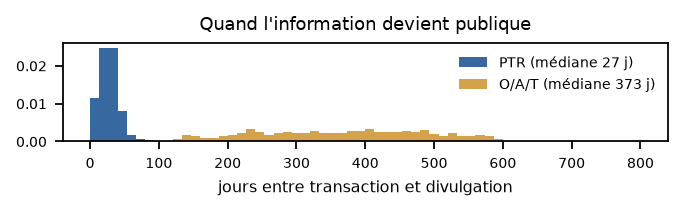
\includegraphics[width=0.70\textwidth]{fig_10_delais.png}\\[0.5mm]
  \defl{figure : PTR $=$ déclaration rapide · O/A/T $=$ rapports, amendements et sorties · divulgation $=$ publication}\\[1.5mm]
  \kpi{helec}{27 j}{opération $\rightarrow$ publication, déclaration rapide}\qquad
  \kpi{dataC}{373 j}{le même délai, rapports annuels}\\[0.5mm]
  \defl{délais médians ; au neuvième décile : 49 jours pour les déclarations rapides, 540 pour les rapports annuels}\\[2.5mm]
  {\scriptsize Chaque transaction entre dans le portefeuille reconstruit à sa
  \textbf{date d'opération}, pas à sa date de publication : au moment où le portefeuille bouge,
  personne à l'extérieur ne sait encore que l'opération a eu lieu.}\\[2mm]
  \piege{tout ce qui est mesuré sur cette base est une \textbf{borne haute}, jamais une performance
  atteignable. Rejouer le flux à la date de publication est le prérequis n\textsuperscript{o}1 ---
  il n'est pas simulé aujourd'hui.}
\end{frame}

% ── 10. qui part d'un portefeuille connu ─────────────────────────────────────
\begin{frame}{166 des 408 membres qui tradent démarrent avec un portefeuille reconstruit}
  \centering
  {\footnotesize Pour une stratégie, seul compte le point de départ : un membre dont on connaît
  le patrimoine d'entrée, ou un membre qui démarre \emph{vide}.}\\[5mm]
  \kpi{okgreen}{172}{ont une photo d'entrée exploitable}\quad
  \kpi{okgreen}{166}{portefeuilles réellement injectés}\quad
  \kpi{alertred}{242}{démarrent à patrimoine nul}\\[3mm]
  \defl{la cascade documentaire qui mène à ces 166 (325 photos retenues $\rightarrow$ 243
  initialisables $\rightarrow$ 166 injectées) est détaillée à l'étape 8.}\\[5mm]
  \piege{un membre qui part de zéro n'a pas de position en face de ses ventes et pas de poids
  justes au démarrage. Sa reconstruction n'est pas « moins précise » : elle décrit un autre objet.}
\end{frame}

% ── 12. la taille de l'échantillon ───────────────────────────────────────────
\begin{frame}{La matière ne fournit que onze points annuels}
  \centering
  {\footnotesize Le flux reconstruit couvre \textbf{11 années civiles} : comparer année par année
  ce qu'on reconstruit à une référence ne donnera jamais que \textbf{11 observations}, et d'une
  année à l'autre l'écart mesuré se disperse de \textbf{5,7 \%/an}.}\\[3mm]
  \kpi{helec}{11}{années civiles couvertes}\quad
  \kpi{dataC}{5,7 \%/an}{dispersion de l'écart annuel ($\hat\sigma$)}\quad
  \kpi{alertred}{4,6 \%/an}{écart minimal détectable}\\[3mm]
  \bmaths{seuil du hasard à 11 observations · marge pour 8 chances sur 10 de le voir · dispersion annuelle · nombre d'années}
         {\mathrm{MDE} \;=\; (1{,}81 + 0{,}88)\times \frac{\hat\sigma}{\sqrt{11}} \;=\; 4{,}6\ \%/\text{an}}
  {\footnotesize L'\textbf{écart minimal détectable} est le plus petit écart annuel moyen qu'un
  échantillon de cette taille permet de distinguer du hasard --- ici \textbf{4,6 \%/an}.}\\[2.5mm]
  \piege{c'est une limite de \emph{taille d'échantillon}, connue avant tout test : un écart réel
  de 1 ou 2 \%/an resterait invisible. Ne jamais lire une absence de conclusion comme une preuve
  d'absence.}
\end{frame}

% ── 13. ce que le Schedule A rendrait possible ───────────────────────────────
\begin{frame}{Les rapports annuels couvrent 460 membres, la photo d'entrée seulement 243}
  \centering
  {\footnotesize Les positions des rapports annuels servent aujourd'hui uniquement à
  \emph{vérifier} la reconstruction --- elles sont pourtant un gisement de points de départ
  bien plus large que la photo d'entrée.}\\[2.5mm]
  {\footnotesize\begin{tabular}{l r r}
    \toprule
    & photo d'entrée \emph{H}/\emph{C} & rapport annuel \emph{O}\\
    \midrule
    documents retenus                 & 325 \defl{(une par membre)} & 4\,447\\
    documents exploitables            & \textbf{261} & \textbf{2\,263}\\
    membres couverts                  & \textbf{243} initialisables & \textbf{460}\\
    lignes valorisées avec un prix    & 7\,782 lignes de départ construites & 43\,019\\
    à quel moment                     & une fois, à l'entrée en mandat & une fois par année de mandat\\
    \bottomrule
  \end{tabular}}\\[2.5mm]
  {\footnotesize \textbf{814} membres ont déposé au moins un rapport annuel, \textbf{460}
  seulement en ont un \emph{exploitable} (tickérisé, valorisé, avec cours) ; le taux de couverture
  médian des années de mandat vaut \textbf{85 \%} (212 membres à 100 \%, 79 à 0 \%).}\\[2mm]
  \choixbox{ce n'est pas fait : le juge doit rester indépendant de ce qu'il juge. Utiliser les
  rapports annuels comme point de départ oblige à trouver un autre juge --- la photo de sortie
  \emph{T} (136 confrontations seulement) est la seule réserve disponible.}
\end{frame}

% ── 14. carte des chiffres 1/4 — les documents ───────────────────────────────
\begin{frame}{La carte des chiffres (1/4) --- les documents et les lignes de patrimoine}
  \centering
  {\footnotesize
  \begin{tabular}{@{}p{0.95\textwidth}@{}}
  \toprule
  \textbf{LES DOCUMENTS DE PATRIMOINE, une fois l'OCR rebranché}\\
  \quad 14\,887 documents portant des lignes de patrimoine $=$ 12\,459 électroniques $+$ 2\,428 océrisés\\
  \quad l'inventaire des photos \emph{datées et rattachées à un membre} n'en retient que 6\,135
        $=$ 4\,447 rapports annuels $+$ 934 candidatures $+$ 378 sorties $+$ 376 entrées\\
  \quad \defl{à ne pas confondre avec le journal de traitement, qui compte tous les documents reçus :
        934 candidatures datées contre 10\,116 documents C au journal, dont 4\,515 lus sans aucune ligne et 1\,583 jamais océrisés}\\
  \quad à côté : 5\,571 dépôts de déclarations rapides \defl{(paires membre × date de divulgation ; 8\,267 documents au journal)}
        · 139 amendements qui déclarent un achat ou une vente\\
  \midrule
  \textbf{LES LIGNES DE PATRIMOINE (\emph{Schedule A})}\\
  \quad 609\,886 lignes $=$ 420\,916 électroniques $+$ 188\,970 océrisées\\
  \quad par type de dépôt : 244\,759 candidature $+$ 238\,624 annuel $+$ 82\,667 amendement
        $+$ 22\,661 entrée $+$ 21\,175 sortie $=$ 609\,886\\
  \quad par nature : 337\,593 sans ticker $+$ 231\,426 actions/ETF $+$ 38\,885 fonds
        $+$ 1\,106 monétaires $+$ 876 faux tickers $=$ 609\,886\\
  \bottomrule
  \end{tabular}}
\end{frame}

% ── 15. carte des chiffres 2/4 — la valeur et les lignes de transactions ─────
\begin{frame}{La carte des chiffres (2/4) --- la valeur et les lignes de transactions}
  \centering
  {\footnotesize
  \begin{tabular}{@{}p{0.95\textwidth}@{}}
  \toprule
  \textbf{LA VALEUR, ET LE PIÈGE DE L'EMPILEMENT}\\
  \quad 104\,130\,M\$ $=$ 87\,405 sans ticker $+$ 12\,790 actions/ETF $+$ 3\,752 fonds
        $+$ 99 monétaires $+$ 84 faux tickers\\
  \quad mais le \emph{stock daté} --- dernier document de chaque membre --- ne vaut que
        8\,887\,M\$ sur 42\,522 lignes, chez 887 déposants : rapport 12$\times$\\
  \midrule
  \textbf{LES LIGNES DE TRANSACTIONS (\emph{Schedule B} et déclarations rapides)}\\
  \quad table de départ 134\,464 $=$ 122\,814 Chambre $+$ 11\,650 Sénat\\
  \quad \emph{Schedule B} des rapports 110\,147 $=$ 84\,032 déjà dites par une déclaration rapide (76 \%) $+$ 26\,115 inédites\\
  \quad ces 26\,115 $=$ 16\,062 négociables $+$ 9\,393 fonds $+$ 364 monétaires $+$ 296 faux tickers\\
  \bottomrule
  \end{tabular}}
\end{frame}

% ── 16. carte des chiffres 3/4 — les transactions retenues ──────────────────
\begin{frame}{La carte des chiffres (3/4) --- les transactions retenues}
  \centering
  {\footnotesize
  \begin{tabular}{@{}p{0.95\textwidth}@{}}
  \toprule
  \textbf{LES TRANSACTIONS RETENUES --- le flux unifié \emph{F}}\\
  \quad \textbf{129\,538} trades $=$ 107\,976 déclarations rapides $+$ 14\,084 rapports annuels
        électroniques $+$ 7\,478 \emph{Schedule B} océrisé\\
  \quad les rapports annuels au sens large pèsent 14\,084 $+$ 7\,478 $=$ 21\,562 trades, soit 16,6 \% du flux\\
  \quad chemin des déclarations rapides : 122\,814 $\rightarrow$ 122\,809 (5 hors fenêtre)
        $\rightarrow$ 107\,976 (14\,833 sans cours) \defl{--- 14\,834 lignes sans cours sur les 122\,814 de départ}\\
  \quad chemin des rapports annuels : 26\,115 $-$ 221 échanges $-$ 14 dates $-$ 290 faux tickers
        $-$ 364 monétaires $-$ 9\,345 fonds $-$ 43 séries corrompues $-$ 1\,275 sans cours
        $-$ 479 doublons $=$ 14\,084\\
  \quad chemin du \emph{Schedule B} océrisé : 155\,306 $\rightarrow$ 51\,859 candidates
        $\rightarrow$ 50\,388 rattachées à un membre du registre \defl{($-$1\,471 non rattachées)}
        $\rightarrow$ 9\,581 sans écho d'une déclaration rapide
        $\rightarrow$ 7\,478 après déduplication \defl{($-$2\,103 doublons internes)}\\
  \bottomrule
  \end{tabular}}
\end{frame}

% ── 17. carte des chiffres 4/4 — membres et portefeuilles ────────────────────
\begin{frame}{La carte des chiffres (4/4) --- les membres et les portefeuilles}
  \centering
  {\footnotesize
  \begin{tabular}{@{}p{0.95\textwidth}@{}}
  \toprule
  \textbf{LES MEMBRES --- le registre de 900}\\
  \quad 900 $=$ 305 vus par les déclarations rapides $+$ 103 vus seulement par les rapports annuels
        $+$ 492 sans aucun trade exploitable\\
  \quad ces 103 $=$ 86 vus par le flux électronique des rapports $+$ 17 apportés par le
        \emph{Schedule B} océrisé\\
  \quad les 408 qui tradent $=$ 172 avec photo d'entrée exploitable $+$ 236 sans photo
        \defl{(et 166 photos réellement injectées, donc 242 départs à patrimoine nul)}\\
  \quad par équipement : 492 rien $+$ 219 partiel $+$ 121 photo\,$+$\,trades\,$+$\,annuels
        $+$ 49 dossier complet $+$ 19 trades seuls $=$ 900\\
  \quad par trajectoire : 314 déjà-là partis $+$ 312 arrivés restés $+$ 149 cycle complet
        $+$ 125 déjà-là restés $=$ 900\\
  \midrule
  \textbf{LES PORTEFEUILLES DE DÉPART}\\
  \quad 325 photos retenues $=$ 291 re-sélectionnées sur les deux origines $+$ 34 conservées de la version précédente\\
  \quad 325 $-$ 64 rien de négociable $-$ 18 aucun cours $=$ 243 initialisables
        $=$ 166 injectées $+$ 77 sans trade à simuler\\
  \quad valeur : 11\,480 lignes d'actions (595\,M\$), dont 84,5 \% converti en parts sur 7\,782 lignes\\
  \bottomrule
  \end{tabular}}
\end{frame}

% ── 16. clôture ──────────────────────────────────────────────────────────────
\begin{frame}{Ce qu'on a entre les mains}
  \centering
  \tuile{helec}{129\,538}{transactions valorisées}
  \tuile{helec}{408}{membres qui tradent}
  \tuile{okgreen}{243}{portefeuilles construits, 166 injectés}
  \tuile{okgreen}{57 \%}{des positions déclarées retrouvées}\\[5mm]
  {\footnotesize
  \textbf{Ce qui est solide} --- le flux de transactions : 129\,538 trades décomposables ligne à
  ligne, chez 408 membres, avec un livre de comptes qui boucle à chaque étape.\\[1.5mm]
  \textbf{Ce qui est partiel} --- le patrimoine : 243 portefeuilles de départ construits sur
  900 membres, et un juge indépendant qui retrouve 57 \% des positions déclarées, en médiane
  sur 1\,878 photos confrontées.\\[1.5mm]
  \textbf{Ce qui manque} --- l'horloge : tout est rejoué à la date d'opération, jamais à la date
  de publication.}\\[4mm]
  \repband{on a un flux de transactions complet et traçable, un point de départ pour 166 des
  408 membres qui tradent, et une reconstruction qui retrouve un peu plus d'une position déclarée
  sur deux. Ce qui manque pour tester une stratégie n'est pas du volume : c'est le décalage de
  publication --- 27 jours sur les déclarations rapides, 373 sur les rapports annuels --- et un
  échantillon plus long que onze années.}
\end{frame}

\end{document}
